%% 
%%  An UIT Edition example
%% 
%%  Example 04-27-26 on page 146.
%% 
%%  Copyright (C) 2012 Vo\ss 
%% 
%%  It may be distributed and/or modified under the conditions
%%  of the LaTeX Project Public License, either version 1.3
%%  of this license or (at your option) any later version.
%% 
%%  See http://www.latex-project.org/lppl.txt for details.
%% 

% Show page(s) 1,2,3

%% ==== 
\PassOptionsToClass{}{beamer}
\documentclass[aspectratio=169]{beamer}
\usepackage[utf8]{inputenc}

%\StartShownPreambleCommands
\usepackage{amsmath,esint}
\usepackage[british]{babel}
\usetheme{Warsaw}
\usecolortheme{rose}

%\usetheme{metropolis}
%\usepackage{appendixnumberbeamer}

%\StopShownPreambleCommands
\usepackage{pgfplots}
\usepackage{ mathrsfs }
\usepackage{caption}

\usepackage{gensymb}
\usepackage{color}
\usepackage{url}
\usetikzlibrary{shapes,backgrounds,calc}

\usepackage{tkz-euclide}
\usetkzobj{all}
\usepackage{tkz-fct}  
\usetikzlibrary{calc}
\usepackage{tikz,calc}

\usepackage[ruled]{algorithm2e}
\usepackage{tikz}
\usetikzlibrary{arrows.meta}
\usepackage{animate}
\DeclareMathOperator*{\minimize}{minimize}

\addtobeamertemplate{navigation symbols}{}{%
    \usebeamerfont{footline}%
    \usebeamercolor[fg]{footline}%
    \hspace{1em}%
    \insertframenumber/\inserttotalframenumber
}

\renewcommand{\thealgocf}{}

\makeatletter
\newcommand\titlegraphicii[1]{\def\inserttitlegraphicii{#1}}
\titlegraphicii{}
\setbeamertemplate{title page}
{
  \vspace{0.3in}
  \vbox{}
   %{\usebeamercolor[fg]{titlegraphic}\inserttitlegraphic\hfill\inserttitlegraphicii\par}
  \begin{centering}
    \begin{beamercolorbox}[sep=8pt,center]{title}
      \usebeamerfont{title}\inserttitle\par%
      \ifx\insertsubtitle\@empty%
      \else%
        \vskip0.25em%
        {\usebeamerfont{subtitle}\usebeamercolor[fg]{subtitle}\insertsubtitle\par}%
      \fi%     
    \end{beamercolorbox}%
    \vskip1em\par
    \begin{beamercolorbox}[sep=8pt,center]{date}
      \usebeamerfont{date}\insertdate
    \end{beamercolorbox}%\vskip0.5em
    \begin{beamercolorbox}[sep=8pt,center]{author}
      \usebeamerfont{author}\insertauthor
    \end{beamercolorbox}
    \begin{beamercolorbox}[sep=8pt,center]{institute}
      \usebeamerfont{institute}\insertinstitute
    \end{beamercolorbox}
  \end{centering}
  %\vfill
}
\makeatother
%\author{Anirban Laha and Preksha Nema \\\vspace{0.2in} Presented By: Mitesh M. Khapra}
\author{Mitesh M. Khapra}
\title{CS7015 (Deep Learning) : Lecture 3}
\subtitle{Sigmoid Neurons, Gradient Descent, Feedforward Neural Networks, Representation Power of Feedforward Neural Networks}
\institute{Department of Computer Science and Engineering\\ Indian Institute of Technology Madras}
\date{January 13, 2017}
\titlegraphic{
\includegraphics[height=1cm,width=2cm]{images/iitm_logo.png}}
%\titlegraphicii{\includegraphics[height=1cm,width=2cm]{logo2}}


\begin{document}


\renewcommand{\thefootnote}{$\star$} 

\tikzset{
    o/.style={
        shorten >=#1,
        decoration={
            markings,
            mark={
                at position 1
                with {
                    \draw circle [radius=#1];
                }
            }
        },
        postaction=decorate
    },
    o/.default=2pt
}

\newcommand\derivative[5]{%
    \tkzDefPointByFct[draw](#1) \tkzGetPoint{start}
  \tkzDefPointByFct[draw](#2) \tkzGetPoint{end}
  \draw[thin,|-|,yshift=-3pt] (start) -- node[black,fill=white,#5] {#3}(start-|end);  
  \draw[thin,|-|,xshift=3pt] (start-|end) -- node[black,fill=white,right] {#4}(end); 
  %\draw[thin] (start) --(end); 
}

\title{Lecture 3}
\author{Mitesh M. Khapra}
\maketitle




%\begin{frame}
%\begin{block}{The story so far ...}
%\begin{itemize}
%\item<1-> Networks of the form that we just saw (containing, an input, output and one or more hidden layers) are called Multilayer Perceptrons (MLP, in short)
%\item<2-> More appropriate terminology would be``Multilayered Network of Perceptrons'' but MLP is the more commonly used term
%\item<3-> The theorem that we just saw gives us the representation power of a MLP with a single hidden layer
%\item<4-> Specifically, it tells us that a MLP with a single hidden layer can represent \textbf{any} boolean function
%\end{itemize}
%\end{block}
%\end{frame}

\begin{frame}
\begin{block}{The story ahead ...}
\begin{itemize}
\item<1-> Enough about boolean functions!
\item<2-> What about arbitrary functions of the form $y=f(x)$ where $x\in \mathbb{R}^n$ (instead of $\{0, 1\}^n$) and $y \in \mathbb{R}$ (instead of $\{0, 1\}$) ?
\item<3-> Can we have a network which can (approximately) represent such functions ?
\item<4-> Before answering the above question we will have to first graduate from \textbf{\textit{perceptrons}} to \textbf{\textit{sigmoidal neurons}} ...
\end{itemize}
\end{block}
\end{frame}

\begin{frame}
\begin{block}{Recall}

\begin{itemize}
\item A perceptron will fire if the weighted sum of its inputs is greater than the threshold (-$w_0$)

\end{itemize}
\end{block}
\end{frame}


\begin{frame}
\begin{columns}

\column{0.4\textwidth}
\begin{overlayarea}{\textwidth}{\textheight}
\begin{center}

\tikzstyle{input_neuron}=[circle,draw=red!50,fill=orange!10,thick,minimum size=1mm]
\tikzstyle{hidden_neuron}=[circle,draw=blue!50,fill=blue!10,thick,minimum size=10mm]
\tikzstyle{output_neuron}=[circle,draw=green!50,fill=green!20,thick,minimum size=4mm]

\tikzstyle{input}=[circle,draw=black!50,fill=black!20,thick,minimum size=.2mm]

\begin{tikzpicture}
\node (input2) at (10,-0.1)  {$x_{1}$};

\node [hidden_neuron] (neuron1) at (10,2)  {};

\node (output0)  at (10,3.5) {$y$};

\draw [->] (input2) -- (neuron1);

\draw [->] (neuron1) -- (output0);

\node (bias) at (8, 2) {$bias = w_0 = -0.5$};
\node (weight) at (9.4,0.6) {$w_1 = 1$};
\onslide<3->{\node (text) at (10,-0.7) {$criticsRating$};}
\end{tikzpicture}

%\end{center}

\end{center}

\end{overlayarea}

\column{0.6\textwidth}
\begin{overlayarea}{\textwidth}{\textheight}
\begin{itemize}
\item<1-> The thresholding logic used by a perceptron is very harsh !
\item<2-> For example, let us return to our problem of deciding whether we will like or dislike a movie
\item<3-> Consider that we base our decision only on one input ($x_1 = criticsRating$ which lies between 0 and 1)
\item<4-> If the threshold is 0.5 ($w_0 = -0.5$) and $w_1 = 1$ then what would be the decision for a movie with $criticsRating=0.51$ ? \onslide<5->{(like)}
\item<6-> What about a movie with $criticsRating=0.49$ ? \onslide<7->{(dislike)}
\item<8-> It seems harsh that we would like a movie with rating 0.51 but not one with a rating of 0.49
\end{itemize}
\end{overlayarea}
\end{columns}
\end{frame}

\begin{frame}
\begin{columns}

\column{0.4\textwidth}
\begin{overlayarea}{\textwidth}{\textheight}
\begin{center}

\only<2->{
\begin{tikzpicture}[scale=0.75]
    \begin{axis}[
        xmin=-2.5, xmax=2.5,
        ymin=-0.0, ymax=1.1,
        axis lines=left,
        xtick=\empty, ytick={1},
        axis on top=true,
        line width = 2pt,
        %domain=-2.5:2.5,
        ylabel=$y$,
        xlabel=$\sum_{i=1}^{n} w_i x_i$,
        label style={scale=2}
        ]

        \addplot[line width = 5pt, domain=-2.5:0,blue] {0};
        \addplot[line width = 2pt, domain=-0.02:2.5,blue] {1};

        \only<5->{\addplot [smooth,line width = 2pt, mark=none,draw=red] {1/(1+exp(-2.5*\x)};}

        \draw[line width=2pt, blue] (axis cs:0,0) -- (axis cs:0,1);
        %% Add the asymptotes
    \end{axis}

        \node at (3.5,-0.5) {-$w_0$};
        %\node at (4.5,3.5) {$\frac{1}{1 + e^{-(\sum_{i=1}^{n} w_i x_i + w_0)}}$};
\end{tikzpicture}
}
%\end{center}

\end{center}

\end{overlayarea}

\column{0.6\textwidth}
\begin{overlayarea}{\textwidth}{\textheight}
\only<1-4>{
\begin{itemize}

\item<1-> This behavior is not a characteristic of the specific problem we chose or the specific weight and threshold that we chose
\item<2-> It is a characteristic of the perceptron function itself which behaves like a step function
\item<3-> There will always be this sudden change in the decision (from 0 to 1) when $\sum_{i=1}^{n} w_i x_i$ crosses the threshold (-$w_0$)
\item<4-> For most real world applications we would expect a smoother decision function which gradually changes from 0 to 1
\end{itemize}
}


\only<5->{
\begin{itemize}
\item<5-> Introducing sigmoid neurons where the output function is much smoother than the step function
\item<6-> Here is one form of the sigmoid function called the logistic function
\only<6->{
\begin{align*}
y = \frac{1}{1 + e^{-(w_0 + \sum_{i=1}^{n} w_i x_i)}}
\end{align*}
}
\item<7-> We no longer see a sharp transition around the threshold -$w_0$
\item<8-> Also the output $y$ is no longer binary but a real value between 0 and 1 which can be interpreted as a probability
\item<9-> Instead of a like/dislike decision we get the probability of liking the movie


\end{itemize}
}

\end{overlayarea}
\end{columns}
\end{frame}


\begin{frame}
\begin{columns}

\column{0.4\textwidth}
\begin{overlayarea}{\textwidth}{\textheight}
\vspace{+0.2in}
\begin{center}
\textbf{Perceptron}
\tikzstyle{input_neuron}=[circle,draw=red!50,fill=orange!10,thick,minimum size=1mm]
\tikzstyle{hidden_neuron}=[circle,draw=blue!50,fill=blue!10,thick,minimum size=10mm]
\tikzstyle{output_neuron}=[circle,draw=green!50,fill=green!20,thick,minimum size=4mm]

\tikzstyle{input}=[circle,draw=black!50,fill=black!20,thick,minimum size=.2mm]

\begin{tikzpicture}
\node (input0) at (8,-0.1)  {$x_{1}$};
\node (input1) at (9,-0.1)  {$x_{2}$};
\node (input2) at (10,-0.1)  {$..$};
\node (input3) at (11,-0.1)  {$..$};
\node (input4) at (12,-0.1)  {$x_{n}$};
\node (input5) at (7,-0.1)  {$x_{0}=1$};

\node [hidden_neuron] (neuron1) at (10,2)  {};


\node (output0)  at (10,3.5) {$y$};

\draw [->] (input0) -- (neuron1);
\draw [->] (input1) -- (neuron1);
\draw [->] (input2) -- (neuron1);
\draw [->] (input3) -- (neuron1);
\draw [->] (input4) -- (neuron1);
\draw [->] (input5) -- (neuron1);

\draw [->] (neuron1) -- (output0);

\node (formula)[scale=.8] at (8.4,0.6) {$w_{1}$};
\node (formula)[scale=.8] at (9.1,0.6) {$w_{2}$};
\node (formula)[scale=.8] at (9.8,0.6) {$..$};
\node (formula)[scale=.8] at (10.4,0.6) {$..$};
\node (formula)[scale=.8] at (11.1,0.6) {$w_{n}$};
\node (formula)[scale=.8] at (7.2,0.6) {$w_{0} = -\theta$};

\end{tikzpicture}

\end{center}
\vspace{-0.2in}
\begin{align*}
y &=1 \quad if \sum^{n}_{i=0} w_i * x_i \geq 0 \\
&=0  \quad if \sum^{n}_{i=0} w_i * x_i < 0
\end{align*}

\end{overlayarea}

\column{0.6\textwidth}
\begin{overlayarea}{\textwidth}{\textheight}
\vspace{+0.2in}
\begin{center}
\textbf{Sigmoid (logistic) Neuron}
\tikzstyle{input_neuron}=[circle,draw=red!50,fill=orange!10,thick,minimum size=1mm]
\tikzstyle{hidden_neuron}=[circle,draw=blue!50,fill=blue!10,thick,minimum size=10mm]
\tikzstyle{output_neuron}=[circle,draw=green!50,fill=green!20,thick,minimum size=4mm]

\tikzstyle{input}=[circle,draw=black!50,fill=black!20,thick,minimum size=.2mm]

\begin{tikzpicture}
\node (input0) at (8,-0.1)  {$x_{1}$};
\node (input1) at (9,-0.1)  {$x_{2}$};
\node (input2) at (10,-0.1)  {$..$};
\node (input3) at (11,-0.1)  {$..$};
\node (input4) at (12,-0.1)  {$x_{n}$};
\node (input5) at (7,-0.1)  {$x_{0}=1$};

\node [hidden_neuron] (neuron1) at (10,2)  {$\sigma$};


\node (output0)  at (10,3.5) {$y$};

\draw [->] (input0) -- (neuron1);
\draw [->] (input1) -- (neuron1);
\draw [->] (input2) -- (neuron1);
\draw [->] (input3) -- (neuron1);
\draw [->] (input4) -- (neuron1);
\draw [->] (input5) -- (neuron1);

\draw [->] (neuron1) -- (output0);

\node (formula)[scale=.8] at (8.4,0.6) {$w_{1}$};
\node (formula)[scale=.8] at (9.1,0.6) {$w_{2}$};
\node (formula)[scale=.8] at (9.8,0.6) {$..$};
\node (formula)[scale=.8] at (10.4,0.6) {$..$};
\node (formula)[scale=.8] at (11.1,0.6) {$w_{n}$};
\node (formula)[scale=.8] at (7.2,0.6) {$w_{0} = -\theta$};

\end{tikzpicture}

\end{center}
\vspace{-0.2in}
\begin{align*}
y = \frac{1}{1 + e^{-(\sum_{i=0}^{n} w_i x_i)}}
\end{align*}
\end{overlayarea}
\end{columns}
\end{frame}



\begin{frame}
\begin{columns}

\column{0.5\textwidth}
\begin{overlayarea}{\textwidth}{\textheight}

\begin{center}
Perceptron
\begin{tikzpicture}[scale=0.75]
    \begin{axis}[
        xmin=-2.5, xmax=2.5,
        ymin=-0.0, ymax=1.1,
        axis lines=left,
        xtick=\empty, ytick={1},
        axis on top=true,
        line width = 2pt,
        %domain=-2.5:2.5,
        ylabel=$y$,
        xlabel=$\sum_{i=1}^{n} w_i x_i$,
        label style={scale=2}
        ]

        \addplot[line width = 5pt, domain=-2.5:0,blue] {0};
        \addplot[line width = 2pt, domain=-0.02:2.5,blue] {1};


        \draw[line width=2pt, blue] (axis cs:0,0) -- (axis cs:0,1);
        %% Add the asymptotes
    \end{axis}

    \node at (3.5,-0.5) {-$w_0$};
    %\node at (4.5,3.5) {$\frac{1}{1 + e^{-(\sum_{i=1}^{n} w_i x_i + w_0)}}$};
\end{tikzpicture}

Not smooth, not continuous (at $w0$), \textbf{not differentiable}

\end{center}


\end{overlayarea}

\column{0.6\textwidth}
\begin{overlayarea}{\textwidth}{\textheight}
\begin{center}
Sigmoid Neuron

\begin{tikzpicture}[scale=0.75]
    \begin{axis}[
        xmin=-2.5, xmax=2.5,
        ymin=-0.0, ymax=1.1,
        axis lines=left,
        xtick=\empty, ytick={1},
        axis on top=true,
        line width = 2pt,
        %domain=-2.5:2.5,
        ylabel=$y$,
        xlabel=$\sum_{i=1}^{n} w_i x_i$,
        label style={scale=2}
        ]


        \addplot [smooth,line width = 2pt, mark=none,draw=red] {1/(1+exp(-2.5*\x)};

        %% Add the asymptotes
    \end{axis}

    \node at (3.5,-0.5) {-$w_0$};
    %\node at (4.5,3.5) {$\frac{1}{1 + e^{-(\sum_{i=1}^{n} w_i x_i + w_0)}}$};
\end{tikzpicture}

Smooth, continuous, \textbf{differentiable}

\end{center}
\end{overlayarea}
\end{columns}
\end{frame}


\begin{frame}
\begin{columns}

\column{0.4\textwidth}
\begin{overlayarea}{\textwidth}{\textheight}
\vspace{+0.2in}
\begin{center}
\textbf{Sigmoid (logistic) Neuron}
\tikzstyle{input_neuron}=[circle,draw=red!50,fill=orange!10,thick,minimum size=1mm]
\tikzstyle{hidden_neuron}=[circle,draw=blue!50,fill=blue!10,thick,minimum size=10mm]
\tikzstyle{output_neuron}=[circle,draw=green!50,fill=green!20,thick,minimum size=4mm]

\tikzstyle{input}=[circle,draw=black!50,fill=black!20,thick,minimum size=.2mm]

\begin{tikzpicture}
\node (input0) at (8,-0.1)  {$x_{1}$};
\node (input1) at (9,-0.1)  {$x_{2}$};
\node (input2) at (10,-0.1)  {$..$};
\node (input3) at (11,-0.1)  {$..$};
\node (input4) at (12,-0.1)  {$x_{n}$};
\node (input5) at (7,-0.1)  {$x_{0}=1$};

\node [hidden_neuron] (neuron1) at (10,2)  {};


\node (output0)  at (10,3.5) {$y$};

\draw [->] (input0) -- (neuron1);
\draw [->] (input1) -- (neuron1);
\draw [->] (input2) -- (neuron1);
\draw [->] (input3) -- (neuron1);
\draw [->] (input4) -- (neuron1);
\draw [->] (input5) -- (neuron1);

\draw [->] (neuron1) -- (output0);

\node (formula)[scale=.8] at (8.4,0.6) {$w_{1}$};
\node (formula)[scale=.8] at (9.1,0.6) {$w_{2}$};
\node (formula)[scale=.8] at (9.8,0.6) {$..$};
\node (formula)[scale=.8] at (10.4,0.6) {$..$};
\node (formula)[scale=.8] at (11.1,0.6) {$w_{n}$};
\node (formula)[scale=.8] at (7.2,0.6) {$w_{0} = -\theta$};

\end{tikzpicture}

\end{center}


\end{overlayarea}

\column{0.6\textwidth}
\begin{overlayarea}{\textwidth}{\textheight}
\begin{itemize}
\item<1-> What next ?
\item<2-> Well, just as we had an algorithm for learning the weights of a perceptron, we also need a way of learning the weights of a sigmoid neuron 
\item<3-> Before we see such an algorithm we will revisit the concept of \textbf{error} 
\end{itemize}
\end{overlayarea}
\end{columns}
\end{frame}


\begin{frame}
\begin{columns}

\column{0.3\textwidth}
\begin{overlayarea}{\textwidth}{\textheight}
\begin{tikzpicture}
\filldraw[red] (1.717248,1.148263) circle (2pt);%--
\filldraw[blue] (1.022337,1.844630) circle (2pt);
\filldraw[blue] (0.929218,1.449012) circle (2pt);
\filldraw[red] (1.256599,1.328157) circle (2pt);%--
\filldraw[blue] (1.917421,1.041134) circle (2pt);
\filldraw[blue] (1.552910,0.757361) circle (2pt);
\filldraw[red] (0.476688,0.993158) circle (2pt);
\filldraw[blue] (1.139669,1.889055) circle (2pt);
\filldraw[red] (1.994183,1.472244) circle (2pt);%--
\filldraw[red] (0.611827,0.938297) circle (2pt);
\filldraw[blue] (1.954791,0.598560) circle (2pt);
\filldraw[red] (0.113127,1.025315) circle (2pt);
\filldraw[blue] (1.547272,1.235639) circle (2pt);
\filldraw[blue] (1.667688,0.664851) circle (2pt);
\filldraw[blue] (0.108270,0.066074) circle (2pt);%--
\filldraw[red] (1.551238,0.091185) circle (2pt);
\filldraw[red] (0.550644,0.461861) circle (2pt);
\filldraw[blue] (1.326191,1.171462) circle (2pt);
\filldraw[red] (0.285269,0.166320) circle (2pt);
\filldraw[blue] (0.645487,1.900755) circle (2pt);
\filldraw[red] (0.715271,0.514446) circle (2pt);
\filldraw[blue] (0.239037,0.110620) circle (2pt);%--
\filldraw[blue] (1.707163,1.213513) circle (2pt);
\filldraw[blue] (0.663682,1.796715) circle (2pt);
\filldraw[red] (0.512817,0.075660) circle (2pt);
\filldraw[blue] (1.542905,0.897760) circle (2pt);
\filldraw[blue] (1.928409,0.514645) circle (2pt);
\filldraw[blue] (0.430763,1.999726) circle (2pt);
\filldraw[red] (0.411993,0.218422) circle (2pt);
\filldraw[red] (0.951387,0.725352) circle (2pt);
\filldraw[red] (0.001601,1.490619) circle (2pt);
\filldraw[red] (0.983530,0.364934) circle (2pt);
\filldraw[red] (0.612532,0.194346) circle (2pt);
\filldraw[blue] (1.217355,1.773029) circle (2pt);
\filldraw[red] (0.398657,0.261244) circle (2pt);
\filldraw[blue] (0.452156,1.890002) circle (2pt);
\filldraw[red] (0.458527,0.384611) circle (2pt);
\filldraw[blue] (1.977895,1.687690) circle (2pt);
\filldraw[blue] (0.217980,0.748811) circle (2pt);%--
\filldraw[red] (0.075486,1.486788) circle (2pt);
\filldraw[blue] (1.872187,1.761516) circle (2pt);
\filldraw[blue] (1.142016,1.716686) circle (2pt);
\filldraw[blue] (1.411278,1.734101) circle (2pt);
\filldraw[blue] (1.951329,1.101424) circle (2pt);
\filldraw[red] (0.543241,0.052208) circle (2pt);

\draw[thick,->] (-0.5,-0.5) -- (3.5,-0.5);
\draw[thick,->] (-0.5,-0.5) -- (-0.5,3.5);

\onslide<4->{\draw[thick,dashed] (2.374856,-1) -- (-1,3.972960);}
%\draw[thick,->] (1.570462,-1) -- (-1,1.610895);
%\draw[thick,->] (1.227613,-1) -- (-1,4.034407);

%\draw[thick,->] (-1.0,1.95) -- (2.21,-1.0);
%\draw[thick,->] (1.721741,-1.0) -- (-1.0,2.296974);


\end{tikzpicture}

\end{overlayarea}

\column{0.7\textwidth}
\begin{overlayarea}{\textwidth}{\textheight}
\begin{itemize}
\item<1-> Earlier we mentioned that a single perceptron cannot deal with this data because it is not linearly separable
\item<2-> What does ``cannot deal with'' mean?
\item<3-> What would happen if we use a perceptron model to classify this data ?
\item<4-> We would probably end up with a line like this ...
\item<5-> This line doesn't seem to be too bad 
\item<6-> Sure, it misclassifies 3 blue points and 3 red points but we could live with this error in \textbf{most} real world applications
\item<7-> From now on, we will accept that it is hard to drive the error to 0 in most cases and will instead aim to reach the minimum possible error
\end{itemize}
\end{overlayarea}
\end{columns}
\end{frame}


\begin{frame}
This brings us to a typical machine learning setup which has the following components...

\begin{itemize}
\item<2-> \textbf{Data:} $\{x_i, y_i\}_{i=1}^{n}$
\item<3-> \textbf{Model:} Our approximation of the relation between $x$ and $y$. For example, 
\onslide<4->{
\begin{align*}
\onslide<4->{\hat{y} &= \frac{1}{1 + e^{-(w^T x)}}}\\
\onslide<5->{or\quad \hat{y} &= w^T x}\\
\onslide<6->{or\quad \hat{y} &= (w^T x)^2}
\end{align*}
}
\onslide<7->{or just about any function}
\item<8-> \textbf{Parameters:} In all the above cases, $w$ is a parameter which needs to be learned from the data
\item<9-> \textbf{Learning algorithm:} An algorithm for learning the parameters ($w$) of the model (for example, perceptron learning algorithm, gradient descent, etc.)
\item<10-> \textbf{Objective/Loss/Error function:} To guide the learning algorithm \onslide<11->{- the learning algorithm should aim to minimize the loss function}
\end{itemize}
\end{frame}

\begin{frame}
As an illustration, consider our movie example

\begin{itemize}
\item<2-> \textbf{Data:} $\{x_i = movie, y_i = like/dislike\}_{i=1}^{n}$ 
\item<3-> \textbf{Model:} Our approximation of the relation between $x$ and $y$ (the probability of liking a movie). 
\onslide<4->{
\begin{align*}
\onslide<4->{\hat{y} &= \frac{1}{1 + e^{-(w^T x)}}}\\
\end{align*}
}
\vspace{-0.3in}
\item<5-> \textbf{Parameter:} $w$ 
\item<6-> \textbf{Learning algorithm:} Gradient Descent [we will see soon]
\item<7-> \textbf{Objective/Loss/Error function:} \onslide<8->{One possibility is
%\vspace{-0.1in}
\begin{align*}
\onslide<8->{\mathscr{L}(w) = \sum_{i=1}^{n} (\hat{y}_i - y_i)^2} \\
\end{align*}
}
%\vspace{-0.1in}
\onslide<9->{The learning algorithm should aim to find a $w$ which minimizes the above function (squared error between $y$ and $\hat{y}$)} 
\end{itemize}
\end{frame}


\begin{frame}

\begin{columns}

\column{0.4\textwidth}
\begin{overlayarea}{\textwidth}{\textheight}
%\vspace{+0.2in}
\only<1-2>{
\begin{center}
\textbf{Sigmoid (logistic) Neuron}
\tikzstyle{input_neuron}=[circle,draw=red!50,fill=orange!10,thick,minimum size=1mm]
\tikzstyle{hidden_neuron}=[circle,draw=blue!50,fill=blue!10,thick,minimum size=10mm]
\tikzstyle{output_neuron}=[circle,draw=green!50,fill=green!20,thick,minimum size=4mm]

\tikzstyle{input}=[circle,draw=black!50,fill=black!20,thick,minimum size=.2mm]

\begin{tikzpicture}
\node (input0) at (8,-0.1)  {$x_{1}$};
\node (input1) at (9,-0.1)  {$x_{2}$};
\node (input2) at (10,-0.1)  {$..$};
\node (input3) at (11,-0.1)  {$..$};
\node (input4) at (12,-0.1)  {$x_{n}$};
\node (input5) at (7,-0.1)  {$x_{0}=1$};

\node [hidden_neuron] (neuron1) at (10,2)  {$\sigma$};


\node (output0)  at (10,3.5) {$y$};

\draw [->] (input0) -- (neuron1);
\draw [->] (input1) -- (neuron1);
\draw [->] (input2) -- (neuron1);
\draw [->] (input3) -- (neuron1);
\draw [->] (input4) -- (neuron1);
\draw [->] (input5) -- (neuron1);

\draw [->] (neuron1) -- (output0);

\node (formula)[scale=.8] at (8.4,0.6) {$w_{1}$};
\node (formula)[scale=.8] at (9.1,0.6) {$w_{2}$};
\node (formula)[scale=.8] at (9.8,0.6) {$..$};
\node (formula)[scale=.8] at (10.4,0.6) {$..$};
\node (formula)[scale=.8] at (11.1,0.6) {$w_{n}$};
\node (formula)[scale=.8] at (7.2,0.6) {$w_{0} = -\theta$};

\end{tikzpicture}

\end{center}
}

\only<3->{
\begin{center}

\tikzstyle{neuron}=[circle,draw=blue!50,fill=blue!20,thick,minimum size=10mm]
\tikzstyle{input}=[circle,draw=black!50,fill=black!20,thick,minimum size=6mm]
\begin{tikzpicture}
\node [neuron] (neuron0) at (1,6)  {$\sigma$} ;
\node (input1) at (-1,6)  {$x$};
\node (input0) at (-1,5)  {$1$};

\onslide<4->{\node (w) at (-0.25,5.8)  {$w$};}
\onslide<4->{\node (b) at (-0.25,5.2)  {$b$};}

\node (output0) at (3,6)  {$\hat{y} = f(x)$};
\onslide<4->{\node (formula) at (0,4) {$f(x)= \frac{1}{1+e^{-(w\cdot x + b)}}$};}
\draw [->] (input0) -- (neuron0);
\draw [->] (input1) -- (neuron0);
\draw [->] (neuron0) -- (output0);
\end{tikzpicture}
\end{center}
}
\end{overlayarea}
\column{0.6\textwidth}
\begin{overlayarea}{\textwidth}{\textheight}
\begin{itemize}
\item<1-> With this setup in mind, we will now focus on this \textbf{model} and discuss an \textbf{algorithm} for learning the \textbf{parameters} of this model from some given \textbf{data}
\item<2-> $\sigma$ stands for the sigmoid function (logistic function in this case) 
\item<3-> For ease of explanation, we will consider a very simplified version of the model having just 1 input
\item<4-> Further to be consistent with the literature, from now on we will refer to $w_0$ as $b$ (bias)
\item<5-> Lastly, instead of considering the problem of predicting like/dislike we will assume that we want to predict $criticsRating (y)$ given  $imdbRating (x)$ (for no particular reason)
\end{itemize}
\end{overlayarea}
\end{columns}
\end{frame}


\begin{frame}

\begin{columns}

\column{0.5\textwidth}
\begin{overlayarea}{\textwidth}{\textheight}

\begin{center}

\tikzstyle{neuron}=[circle,draw=blue!50,fill=blue!20,thick,minimum size=10mm]
\tikzstyle{input}=[circle,draw=black!50,fill=black!20,thick,minimum size=6mm]
\begin{tikzpicture}
\node [neuron] (neuron0) at (1,6)  {$\sigma$} ;
\node (input1) at (-1,6)  {$x$};
\node (input0) at (-1,5)  {$1$};

\node (w) at (-0.25,5.8)  {$w$};
\node (b) at (-0.25,5.2)  {$b$};

\node (output0) at (3,6)  {$\hat{y} = f(x)$};
\onslide<4->{\node (formula) at (0,4) {$f(x)= \frac{1}{1+e^{-(w\cdot x + b)}}$};}
\draw [->] (input0) -- (neuron0);
\draw [->] (input1) -- (neuron0);
\draw [->] (neuron0) -- (output0);
\end{tikzpicture}
\end{center}



\only<5->{
\vspace{-0.2in}
\begin{figure}[!htp]
\begin{center}
    \includegraphics<5-8>[scale=0.3]{images/2sample_points.png}
    \includegraphics<9->[scale=0.3]{images/2sample_points_sigmoid.png}
\end{center}
\end{figure}
}
\end{overlayarea}

\column{0.5\textwidth}<2->
\begin{overlayarea}{\textwidth}{\textheight}
\only<2-4>{
\begin{block}<2-4>{Input for training}
$\{x_i, y_i\}^{N}_{i=1} \rightarrow N$ pairs of $(x,y)$
\end{block}
\begin{block}<3-4>{Training objective}
Find $w$ and $b$ such that:\\
$\displaystyle{\minimize_{w,b} \mathscr{L}(w,b) = \sum_{i=1}^{N} (y_i - f(x_i))^2}$
\end{block}
}

\only<5->{
\begin{block}{What does it mean to train the network?}
\begin{itemize}
    \item<5-> Suppose we train the network with $ (x, y) = (0.5, 0.2)$ and $(2.5, 0.9)$  
    \item<6-> At the end of training we expect to find w*, b* such that:
    \item<7-> $f(0.5) \rightarrow 0.2$ and  $f(2.5) \rightarrow 0.9$
\end{itemize}

\end{block}

\begin{block}<8->{In other words...}
\begin{itemize}
    \item We hope to find a sigmoid function such that $(0.5, 0.2)$ and $(2.5, 0.9)$ lie on this sigmoid
\end{itemize}
\end{block}

}
\end{overlayarea}
\end{columns}
\end{frame}

%\subsection{Curve-fitting}
\begin{frame}
\fontsize{16pt}{7.2}\selectfont
 \textit{Lets see this in more detail....}
\end{frame}

\begin{frame}
\begin{columns}
\column{0.35\textwidth}
\begin{overlayarea}{\textwidth}{\textheight}
\begin{onlyenv}<1->
\begin{figure}[!htp]
  \begin{center}
    \includegraphics<1-2>[scale=0.3]{images/2sample_points.png}
    \includegraphics<3-11>[scale=0.3]{images/random/sig0.png}
    \includegraphics<12>[scale=0.3]{images/random/sig1.png}
    \includegraphics<13>[scale=0.3]{images/random/sig2.png}
    \includegraphics<14>[scale=0.3]{images/random/sig3.png}
    \includegraphics<15>[scale=0.3]{images/random/sig4.png}
    \includegraphics<16->[scale=0.3]{images/random/sig5.png}
  \end{center}
\end{figure}  
\end{onlyenv}
\end{overlayarea}

\column{0.65\textwidth}
\begin{overlayarea}{\textwidth}{\textheight}
\only<2-5>{
\begin{itemize}
    \item Can we try to find such a $w*, b*$ manually
    \item<3-> Lets try a random guess.. (say, $w=0.5, b=0$)
    \item<4-> Clearly not good, but how bad is it ?
    \item<5-> Lets revisit $\mathscr{L}(w,b)$ to see how bad it is ... 
\end{itemize}
}

\only<6-10>{
\begin{align*}
 \onslide<6->{\mathscr{L}(w,b) &= \frac{1}{2} * \sum_{i=1}^{N} (y_i - f(x_i))^2}   \\
 \onslide<7->{&= \frac{1}{2} * (y_1 - f(x_1))^2 + (y_2 - f(x_2))^2} \\
 \onslide<8->{&= \frac{1}{2} * (0.9 - f(2.5))^2 + (0.2 - f(0.5))^2} \\
 \onslide<9->{&= 0.073}
\end{align*}
\only<10->{\parbox[c][50pt][c]{230pt}{We want $\mathscr{L}(w,b)$ to be as close to 0 as possible}}
}

\only<11-> {
Lets try some other values of w, b 

\begin{flushleft}
\begin{table}
\begin{tabular}{ccc}
\hline
\hline
$w$&$b$&$\mathscr{L}(w,b)$\\
\hline
\hline
0.50&0.00& 0.0730 \\
\only<12-> {-0.10 & 0.00 & 0.1481} \\
\only<13-> {0.94 & -0.94 & 0.0214}\\
\only<14-> {1.42 & -1.73 & 0.0028}\\
\only<15-> {1.65 & -2.08 & 0.0003}\\
\only<16-> {1.78 &-2.27 & 0.0000}\\
\hline
\hline
\end{tabular}
\end{table}
\end{flushleft}

\only<12>{\parbox[c][50pt][c]{230pt}{Oops!! this made things even worse...}}
\only<13>{\parbox[c][50pt][c]{230pt}{Perhaps it would help to push w and b in the other direction...}}
\only<14-15>{\parbox[c][50pt][c]{230pt}{Lets keep going in this direction, \textit{i.e.}, increase $w$ and decrease $b$}}
\only<16>{\parbox[c][50pt][c]{230pt}{With some guess work and intuition we were able to find the right values for $w$ and $b$}}
}
\end{overlayarea}
\end{columns}

\end{frame}

%\subsection{Error surfaces}
\begin{frame}
\fontsize{16pt}{7.2}\selectfont
 \textit{Lets look at something better than our ``guess work'' algorithm....}
\end{frame}

\begin{frame}
\begin{columns}
\column{0.5\textwidth}
\begin{overlayarea}{\textwidth}{\textheight}
\begin{onlyenv}<1->
\begin{figure}[!htp]
  \begin{center}
    \includegraphics<2->[scale=0.5]{images/error_surface1.png}
  \end{center}
\end{figure}  
\end{onlyenv}
\end{overlayarea}

\column{0.5\textwidth}
\begin{overlayarea}{\textwidth}{\textheight}
\begin{itemize}
    \item Since we have only 2 points and 2 parameters ($w$, $b$) we can easily plot $\mathscr{L}(w,b)$ for different values of ($w$, $b$) and pick the one where $\mathscr{L}(w,b)$ is minimum
    \item<3-> But of course this becomes intractable once you have many more data points and many more parameters !!
    \item<4-> Further, even here we have plotted the error surface only for a small range of ($w$, $b$) [from $(-6, 6)$ and not from $(-\inf, \inf)$]
\end{itemize}
\end{overlayarea}
\end{columns}
\end{frame}

\begin{frame}
\fontsize{16pt}{7.2}\selectfont
 \textit{Lets look at the geometric interpretation of our ``guess work'' algorithm in terms of this error surface}
\end{frame}


\begin{frame}
\begin{columns}
\column{0.5\textwidth}
\begin{overlayarea}{\textwidth}{\textheight}
\begin{onlyenv}<1->
\begin{figure}[!htp]
  \begin{center}
    \includegraphics<1>[scale=0.4]{images/2sample_points.png}
    \includegraphics<2>[scale=0.4]{images/random/sig0.png}
    \includegraphics<3>[scale=0.4]{images/random/sig1.png}
    \includegraphics<4>[scale=0.4]{images/random/sig2.png}
    \includegraphics<5>[scale=0.4]{images/random/sig3.png}
    \includegraphics<6>[scale=0.4]{images/random/sig4.png}
    \includegraphics<7->[scale=0.4]{images/random/sig5.png}
  \end{center}
\end{figure}  
\end{onlyenv}
\end{overlayarea}

\column{0.5\textwidth}
\begin{overlayarea}{\textwidth}{\textheight}
\begin{onlyenv}<1->
\begin{figure}[!htp]
  \begin{center}
    \includegraphics<1>[scale=0.5]{images/error_surface1.png}
    \includegraphics<2>[scale=0.5]{images/random/error0.png}
    \includegraphics<3>[scale=0.5]{images/random/error1.png}
    \includegraphics<4>[scale=0.5]{images/random/error2.png}
    \includegraphics<5>[scale=0.5]{images/random/error3.png}
    \includegraphics<6>[scale=0.5]{images/random/error4.png}
    \includegraphics<7->[scale=0.5]{images/random/error5.png}
  \end{center}
\end{figure}  
\end{onlyenv}
\end{overlayarea}

\end{columns}

\end{frame}


\begin{frame}
\fontsize{16pt}{7.2}\selectfont
 \textit{Now lets see if there is a more efficient and principled way of doing this}
\end{frame}

\section{Optimization methods}
%\subsection{Gradient Descent}
%\subsection{Goal}
\begin{frame}
 \begin{block}{Goal}
     Find a better way of traversing the error surface so that we can reach the minimum value quickly without resorting to brute force search! 
 \end{block}
\end{frame}


\begin{frame}
\begin{overlayarea}{\textwidth}{\textheight}
\begin{tikzpicture}[inner sep=2mm]
\node (theta) at (1,6)  {\only<1->{$\theta = [w, b]$}} ;
\node (deltatheta) at (1,5)  {\only<2->{$\Delta\theta = [\Delta w, \Delta b]$}} ;
\node (thetanew) at (1,3)  {\only<9->{$\theta_{new} = \theta + \eta\cdot\Delta\theta$}} ;
\node (text1) at (-1,7)  {\only<1->{{\parbox[c][20pt][c]{110pt}{vector of parameters, say, randomly initialized}}}};
\node (text2) at (-2,4)  {\only<2->{{\parbox[c][20pt][c]{70pt}{change in the values of w, b}}}};
\node (text3) at (6,2)  {\only<10->{{\parbox[c][20pt][c]{190pt}{\textbf{Question:} What is the right $\Delta\theta$ to use ?}}}};

\node (text4) at (9,6)  {\only<5->{{\parbox[c][40pt][c]{120pt}{We moved in the direction of $\Delta\theta$}}}};

\node (text5) at (9,4)  {\only<6->{{\parbox[c][60pt][c]{120pt}{Lets be a bit conservative: move only by a small amount $\eta$}}}};

\node (text4) at (6,1)  {\only<11->{{\parbox[c][20pt][c]{190pt}{The answer comes from Taylor series}}}};


\only<1->{\draw [->] (text1) to [out=-90,in=180] (theta)};
\only<2->{\draw [->] (text2) to [out=90,in=180] (deltatheta)};
\only<10->{\draw [->] (text3) to [out=90,in=0] (thetanew)};

\only<3->{\draw [->] (3,5) to node[left]{$\theta$} (4,7)};
\only<3->{\draw [->] (3,5) to node[below]{$\Delta\theta$} (6,5)};
\only<4->{\draw [dashed] (4,7) to (7,7)};
\only<4->{\draw [dashed] (6,5) to (7,7)};
\only<4->{\draw [->] (3,5) to node[left]{$\theta_{new}$} (7,7)};

\begin{scope}[color=red]
\only<7->{\draw [->] (3,5) to node[below]{$\eta\cdot\Delta\theta$} (4,5)};
\only<8->{\draw [dashed] (4,7) to (5,7)};
\only<8->{\draw [dashed] (4,5) to (5,7)};
\only<8->{\draw [->] (3,5) to  (5,7)};
\end{scope}
\end{tikzpicture}
\end{overlayarea}

\end{frame}

%\subsection{Taylor series}
\begin{frame}
\begin{overlayarea}{\textwidth}{\textheight}
For ease of notation, let $\Delta\theta = u$, then from Taylor series, we have,

\begin{align*}
        \only<2->{\mathscr{L}(\theta + \eta u) &=  \mathscr{L}(\theta)+ \eta*u^T \nabla\mathscr{L}(\theta) + \frac{\eta^2}{2!}*u^T \nabla^2\mathscr{L}(\theta)u + \frac{\eta^3}{3!}*... + \frac{\eta^4}{4!}*...}\\
        \only<3->{&= \mathscr{L}(\theta)+ \eta*u^T \nabla\mathscr{L}(\theta) \text{  } [\textit{$\eta$ is typically small, so $\eta^2, \eta^3,.. \rightarrow 0$}]}
\end{align*}

\only<4->{Note that the move ($\eta u$) would be favorable only if,}
\begin{align*}
\only<4->{&\mathscr{L}(\theta + \eta u) - \mathscr{L}(\theta) < 0 [\textit{i.e., if the new loss is less than the previous loss}]} \\
\only<5->{\intertext {This implies,}}
\only<5->{&u^T \nabla\mathscr{L}(\theta) < 0}
\end{align*}
\end{overlayarea}
\end{frame}

\begin{frame}

\begin{overlayarea}{\textwidth}{\textheight}
Okay, so we have,
\begin{align*}
u^T \nabla\mathscr{L}(\theta) < 0
\end{align*}

\only<1->{But, what is the range of $u^T \nabla\mathscr{L}(\theta)$ ?} \only<2->{Lets see....}\\

\only<3->{Let $\beta$ be the angle between $u^T$ and $\nabla\mathscr{L}(\theta)$, then we know that,} 
\only<4->{
\begin{align*}
\only<4->{-1 &\leq cos(\beta) = \frac{u^T \nabla\mathscr{L}(\theta)}{||u||*||\nabla\mathscr{L}(\theta)||} \leq 1}
%\only<5->{\intertext{Lets assume $u$ and $\mathscr{L}'(\theta)$ are unit vectors}}
\only<6->{\intertext{multiply throughout by $k = ||u||*||\nabla\mathscr{L}(\theta)||$ }}
\only<6->{-k &\leq k*cos(\beta) = u^T \nabla\mathscr{L}(\theta) \leq k }
\only<7->{\intertext{Thus, $\mathscr{L}(\theta + \eta u) - \mathscr{L}(\theta) = u^T \nabla\mathscr{L}(\theta) = k*cos(\beta)$ will be most negative when $cos(\beta) =-1$ \textit{i.e.}, when $\beta$ is $180\degree$}}
\end{align*}
}

\end{overlayarea}
\end{frame}

%\subsection{The update rule}
\begin{frame}
\begin{overlayarea}{\textwidth}{\textheight}

\begin{block}{Gradient Descent Rule}
\begin{itemize}
    \item<1-> The direction $u$ that we intend to move in should be at $180\degree$ w.r.t. the gradient
    \item<2-> In other words, move in a direction opposite to the gradient
\end{itemize}
\end{block}

\only<3->{
\begin{block}{Parameter Update Equations}
\vspace{-0.1in}
\begin{align*}
    w_{t+1} &= w_{t} - \eta \nabla w_{t} \\
    b_{t+1} &= b_{t} - \eta \nabla b_{t} \\
    where, \nabla w_{t} &= \frac{\partial\mathscr{L}(w,b)}{\partial w}_{\textit{at $w=w_t, b=b_t$}}, 
    \nabla b = \frac{\partial\mathscr{L}(w,b)}{\partial b}_{\textit{at $w=w_t, b=b_t$}}
\end{align*}
\end{block}
}

\only<4-> {So we now have a more principled way of moving in the $w$-$b$ plane than our ``guess work'' algorithm}


\end{overlayarea}
\end{frame}

\begin{frame}
\begin{overlayarea}{\textwidth}{\textheight}

\begin{itemize}
    
\item <1-> Lets create an algorithm from this rule ... 

\only<2-> {
\begin{algorithm}[H]
\SetAlgoLined
$t \leftarrow 0$\; 
$max\_iterations\leftarrow 1000$\;
 \While{$t < max\_iterations$}{
 $w_{t+1} \leftarrow w_{t} - \eta \nabla w_{t}$\;
 $b_{t+1} \leftarrow b_{t} - \eta \nabla b_{t}$\;
  }
 \caption{gradient\_descent()}
\end{algorithm}
}

\item <2-> To see this algorithm in practice lest first derive $\nabla w$ and $\nabla b$ for our toy neural network

\end{itemize}

\end{overlayarea}

\end{frame}

\begin{frame}
\begin{columns}

\column{0.5\textwidth}
\begin{overlayarea}{\textwidth}{\textheight}
\tikzstyle{neuron}=[circle,draw=blue!50,fill=blue!20,thick,minimum size=10mm]
\tikzstyle{input}=[circle,draw=black!50,fill=black!20,thick,minimum size=6mm]
\begin{tikzpicture}
\node [neuron] (neuron0) at (1,6)  {$\sigma$} ;
\node (input1) at (-1,6)  {$x$};
\node (input0) at (-1,5)  {$1$};
\node (output0) at (3,6)  {$y = f(x)$};
\node (formula) at (0,4) {$f(x)= \frac{1}{1+e^{-(w\cdot x + b)}}$};
\draw [->] (input0) -- (neuron0);
\draw [->] (input1) -- (neuron0);
\draw [->] (neuron0) -- (output0);
\end{tikzpicture}

\vspace{-0.2in}
\begin{figure}[!htp]
\begin{center}
    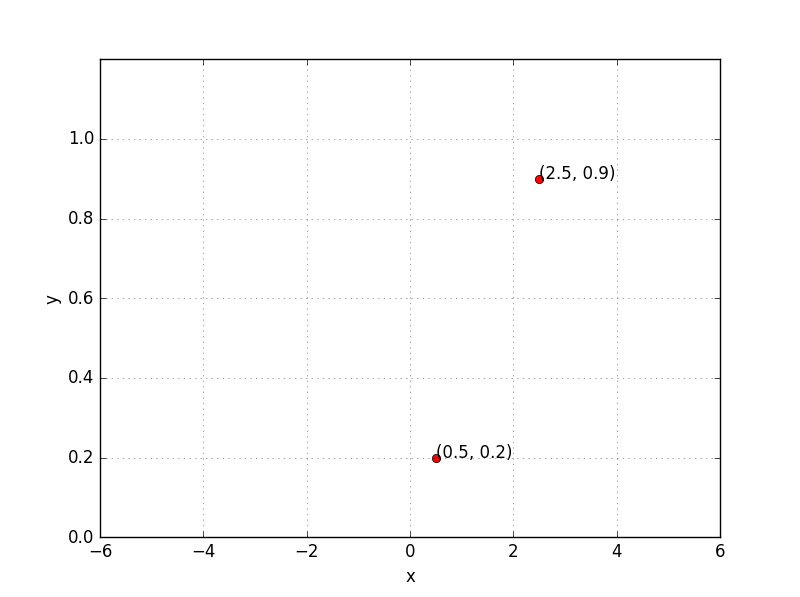
\includegraphics[scale=0.3]{images/2sample_points.png}
\end{center}
\end{figure}

\end{overlayarea}

\column{0.5\textwidth}<2->
\begin{overlayarea}{\textwidth}{\textheight}
\begin{align*}
    \onslide<2->{\intertext{Let's assume there is only 1 point to fit $(x, y)$}}
    \onslide<3->{\mathscr{L}(w,b) &= \frac{1}{2} * (f(x) - y)^2 \\} 
    \onslide<4->{\nabla w = \frac{\partial\mathscr{L}(w,b)}{\partial w} &= \frac{\partial}{\partial w} [\frac{1}{2} * (f(x) - y)^2] \\} 
\end{align*}

\end{overlayarea}
\end{columns}
\end{frame}

\begin{frame}
\begin{columns}
\begin{column}{0.46\textwidth}
\begin{overlayarea}{\textwidth}{\textheight}
\begin{align*}
    \onslide<1->\nabla w &= \frac{\partial}{\partial w} [\frac{1}{2} * (f(x) - y)^2] \\
    \onslide<2->{&= \frac{1}{2} * [2*(f(x) - y) * \frac{\partial}{\partial w}(f(x) - y)] \\}
    \onslide<3->{&= (f(x) - y) * \frac{\partial}{\partial w}(f(x)) \\}
    \onslide<4->{&= (f(x) - y) * \frac{\partial}{\partial w}\Big(\frac{1}{1 + e^{-(wx + b)}}\Big) \\}
    \onslide<10->{ &= \color{red}{(f(x) - y) * f(x)*(1- f(x)) *x}}
\end{align*}
\end{overlayarea}
\end{column}

\vrule{}

\begin{column}{0.54\textwidth}
\begin{overlayarea}{\textwidth}{\textheight}

\begin{align*}
    \onslide<5->{&\frac{\partial}{\partial w}\Big(\frac{1}{1 + e^{-(wx + b)}}\Big) \\}
    \onslide<6->{&=\frac{-1}{(1 + e^{-(wx + b)})^2}\frac{\partial}{\partial w}(e^{-(wx + b)})) \\}
    \onslide<7->{&=\frac{-1}{(1 + e^{-(wx + b)})^2}*(e^{-(wx + b)})\frac{\partial}{\partial w}(-(wx + b))) \\}
    \onslide<8->{&=\frac{-1}{(1 + e^{-(wx + b)})}*\frac{e^{-(wx + b)}}{(1 + e^{-(wx + b)})} *(-x) \\}
    \onslide<8->{&=\frac{1}{(1 + e^{-(wx + b)})}*\frac{e^{-(wx + b)}}{(1 + e^{-(wx + b)})} *(x) \\}
    \onslide<9->{ &=f(x)*(1- f(x))*x}
\end{align*}
\end{overlayarea}
\end{column}

\end{columns}

\end{frame}


\begin{frame}
\begin{columns}

\column{0.45\textwidth}
\begin{overlayarea}{\textwidth}{\textheight}
\tikzstyle{neuron}=[circle,draw=blue!50,fill=blue!20,thick,minimum size=10mm]
\tikzstyle{input}=[circle,draw=black!50,fill=black!20,thick,minimum size=6mm]
\begin{tikzpicture}
\node [neuron] (neuron0) at (1,6)  {$\sigma$} ;
\node (input1) at (-1,6)  {$x$};
\node (input0) at (-1,5)  {$1$};
\node (output0) at (3,6)  {$y = f(x)$};
\node (formula) at (0,4) {$f(x)= \frac{1}{1+e^{-(w\cdot x + b)}}$};
\draw [->] (input0) -- (neuron0);
\draw [->] (input1) -- (neuron0);
\draw [->] (neuron0) -- (output0);
\end{tikzpicture}

\vspace{-0.2in}
\begin{figure}[!htp]
\begin{center}
    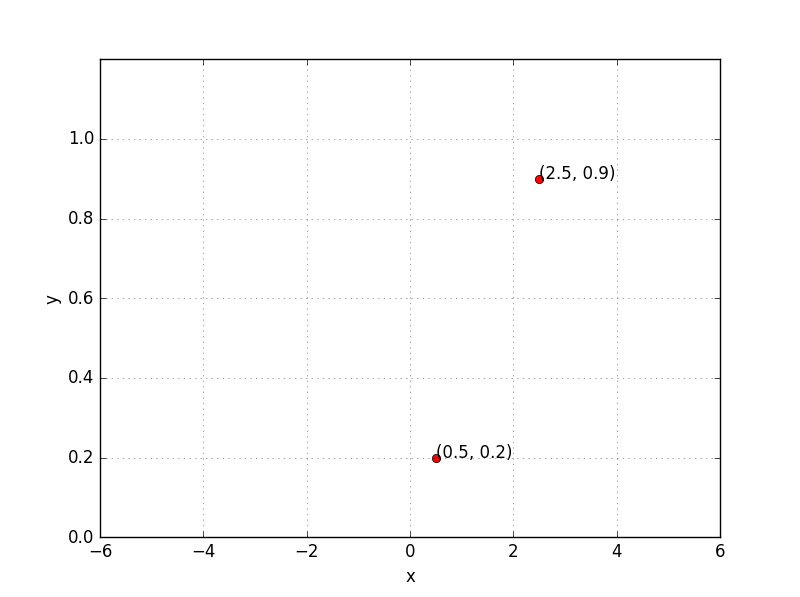
\includegraphics[scale=0.3]{images/2sample_points.png}
\end{center}
\end{figure}

\end{overlayarea}

\column{0.55\textwidth}<1->
\begin{overlayarea}{\textwidth}{\textheight}
\begin{align*}
    \onslide<1->{\intertext{So if there is only 1 point $(x, y)$, we have, }}
    %\only<1->{\mathscr{L}(w,b) &= \frac{1}{2} * (f(x) - y)^2 \\} 
%    \only<1->{\nabla w &= \frac{\partial\mathscr{L}(w,b)}{\partial w} &= \frac{\partial}{\partial w} [\frac{1}{2} * (f(x) - y)^2] \\} 
    \onslide<2->{\nabla w &= (f(x) - y) * f(x)*(1- f(x)) *x} 
    \onslide<3->{\intertext{For two points,}}
    \onslide<4->{\nabla w &= \sum_{i=1}^{2} (f(x_i) - y_i) * f(x_i)*(1- f(x_i)) *x_i} \\
    %\only<5->{\intertext{Similarly}}
    \onslide<5->{\nabla b &= \sum_{i=1}^{2} (f(x_i) - y_i) * f(x_i)*(1- f(x_i))} 
\end{align*}

\end{overlayarea}
\end{columns}
\end{frame}


\begin{frame}
\begin{columns}

\column{0.5\textwidth}
\begin{overlayarea}{\textwidth}{\textheight}
\vspace{-0.15in}
\begin{figure}
    \includegraphics<1>[clip,trim=0 650 0 0,scale=0.3]{images/pseudo_code_sgd_crop.png}
    \includegraphics<2>[clip,trim=0 580 0 0,scale=0.3]{images/pseudo_code_sgd_crop.png}
    \includegraphics<3-4>[clip,trim=0 415 0 0,scale=0.3]{images/pseudo_code_sgd_crop.png}
    \includegraphics<5>[clip,trim=0 325 0 0,scale=0.3]{images/pseudo_code_sgd_crop.png}
    \includegraphics<6>[clip,trim=0 235 0 0,scale=0.3]{images/pseudo_code_sgd_crop.png}
    \includegraphics<7>[scale=0.3]{images/pseudo_code_sgd_crop.png}
\end{figure}
\end{overlayarea}

\column{0.5\textwidth}
\begin{overlayarea}{\textwidth}{\textheight}


\begin{figure}
    \includegraphics<4->[scale=0.5]{images/error_surface1.png}
\end{figure}

%<4>Why are the changes in  w \& b so small ?
%<5>Why do we see larger changes in  w \& b now ?
%<6>And again the changes in  w \& b become small. Why ?
\end{overlayarea}

\end{columns}
\end{frame}


\begin{frame}

\begin{columns}
\column{0.5\textwidth}
\begin{overlayarea}{\textwidth}{\textheight}
\vspace{-0.15in}
\begin{figure}
    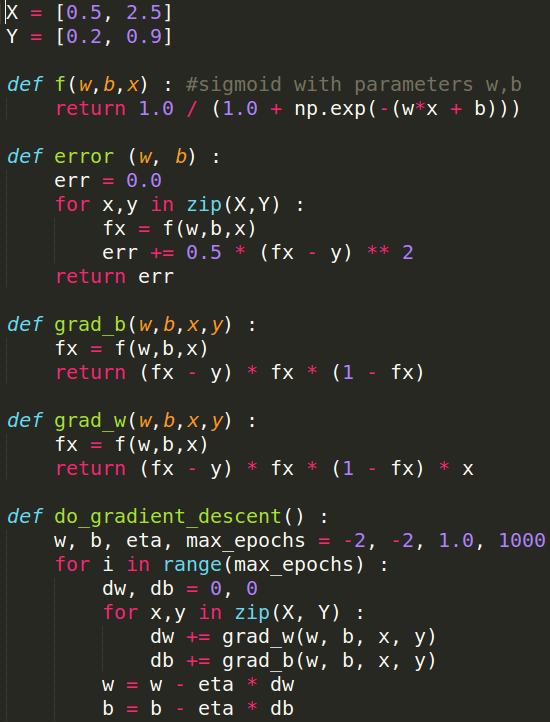
\includegraphics[scale=0.3]{images/pseudo_code_sgd_crop.png}
\end{figure}
\end{overlayarea}

\column{0.5\textwidth}
\begin{overlayarea}{\textwidth}{\textheight}
\vspace{-0.15in}

%\animategraphics[scale=0.5]{12}{images/sgd0/sgd_error}{0}{99}

\begin{figure}
\foreach \n in {0,...,99} {%
    \includegraphics<\n>[scale=0.5]{images/sgd0/sgd_error\n.png}
}
\end{figure}
\end{overlayarea}

\end{columns}
\end{frame}


\begin{frame}
\begin{itemize}
\item<1-> Later on in the course we will look at gradient descent in much more detail and discuss its variants
\item<2-> For the time being it suffices to know that we have an algorithm for learning the parameters of a sigmoid neuron
\item<3-> So where do we head from here ?
\end{itemize}
\end{frame}

%\begin{frame}
%Slide containing the diagrams  and then a `?'
%\end{frame}

\begin{frame}
\begin{columns}
\column{0.5\textwidth}
\begin{overlayarea}{\textwidth}{\textheight}
\textbf{Representation power of a multilayer network of perceptrons}
\vspace{0.1in}

\onslide<2->{\color{blue}{A multilayer network of perceptrons} \color{black}{} with a single hidden layer can be used to \color{cyan}{represent} \color{black}{} any \color{red}{boolean} \color{black}{} function \color{orange}{precisely (no errors)}} %($f(x): \{0, 1\}^n \rightarrow \{0, 1\}^m$) . \\

\end{overlayarea}



\column{0.5\textwidth}
\begin{overlayarea}{\textwidth}{\textheight}
\textbf{Representation power of a multilayer network of sigmoid neurons}
\vspace{0.1in}

\onslide<3->{\color{blue}{A multilayer network of neurons} \color{black}{} with a single hidden layer can be used to \color{cyan}{approximate} \color{black}{} any \color{red}{continuous} \color{black}{} function  \color{orange}{to any desired precision} \color{black}{}} %($f(x): \mathbb{R}^n \rightarrow \mathbb{R}^m$).  \\

\vspace{0.2in}
\onslide<4->{In other words, there is a guarantee that for any function $f(x): \mathbb{R}^n \rightarrow \mathbb{R}^m$, we can always find a neural network (with 1 hidden layer containing enough neurons) whose output g(x) satisfies $|g(x) - f(x) | < \epsilon$ !! \\}
\vspace{0.2in}
%(From now on in this course we will refer to a \textbf{network of neurons} as \textbf{feedforward neural networks} - though in the literature they are often referred to as \textbf{multilayer perceptrons} also) \\

\onslide<5->{\textbf{Proof:} We will see an illustrative proof of this... [Cybenko, 1989], [Hornik, 1991]}
\end{overlayarea}
\end{columns}
\end{frame}


\begin{frame}
\begin{itemize}
\item See this link\footnote{\url{http://neuralnetworksanddeeplearning.com/chap4.html}} for an excellent illustration of this proof 
\item The discussion in the next few slides is based on the ideas presented at the above link
\end{itemize}
\end{frame}

\begin{frame}
\begin{columns}
\column{0.5\textwidth}
\begin{overlayarea}{\textwidth}{\textheight}
\begin{onlyenv}
\begin{figure}
\centering
\includegraphics<1>[scale=0.3]{./images/Plots/plot1}
\includegraphics<2>[scale=0.3]{./images/Plots/plot1_lessbins.png}
\includegraphics<3>[scale=0.3]{./images/Plots/plot1_morebins.png}
\includegraphics<4->[scale=0.4]{./images/Plots/plot1_morebins_detail.png}
\end{figure}
\end{onlyenv}
\end{overlayarea}

\column{0.5\textwidth}
\begin{overlayarea}{\textwidth}{\textheight}
\begin{itemize}
\item We are interested in knowing whether a network of neurons can be used to represent an arbitrary function (like the one shown in the figure)
\item<2-> We observe that such an arbitrary function can be approximated by several ``tower'' functions 
\item<3-> More the number of such ``tower'' functions, better the approximation  
\item<4-> To be more precise, we can approximate any arbitrary function by a sum of such ``tower'' functions 
\end{itemize}
\end{overlayarea}
\end{columns}
\end{frame}

\begin{frame}
\begin{columns}
\column{0.5\textwidth}
\begin{overlayarea}{\textwidth}{\textheight}

\tikzstyle{neuron}=[circle,draw=red!50,fill=red!10, thick,minimum size=10mm]
\tikzstyle{neuron1}=[circle,draw=blue!50,fill=cyan!10, thick,minimum size=10mm]
\begin{tikzpicture}[scale=0.6]

\onslide<3->{
\node [neuron] (neuron1) at (10,0) {$x$};

\draw[->] (neuron1) -- (5.7,1.6);
\draw[->] (neuron1) -- (7.7,1.6);
\node[text width=0.5cm] at (10,1.2) {\LARGE {.}};
\node[text width=0.5cm] at (10.5,1.2) {\LARGE {.}};
\node[text width=0.5cm] at (11,1.2) {\LARGE {.}};
\draw[->] (neuron1) -- (12.7,1.6);
\draw[->] (neuron1) -- (14.7,1.6);


\node[text width=0.5cm] at (5.5,2.5) {Tower maker};
\draw[gray,thick,solid] (5,1.7) rectangle (6.75,3.3);

\node[text width=0.5cm] at (7.5,2.5) {Tower maker};
\draw[gray,thick,solid] (7,1.7) rectangle (8.75,3.3);

\node[text width=0.5cm] at (9.5,2.5) {\LARGE {.}};
\node[text width=0.5cm] at (10.5,2.5) {\LARGE {.}};
\node[text width=0.5cm] at (11.5,2.5) {\LARGE {.}};

\node[text width=0.5cm] at (12.5,2.5) {Tower maker};
\node[text width=0.5cm] at (12.5,2.5) {Tower maker};

\node[text width=0.5cm] at (12.5,2.5) {Tower maker};
\draw[gray,thick,solid] (12,1.7) rectangle (13.75,3.3);

\node[text width=0.5cm] at (14.5,2.5) {Tower maker};
\draw[gray,thick,solid] (14,1.7) rectangle (15.75,3.3);
}

\onslide<4-> {
\node (plot) at (5.7,4.5) {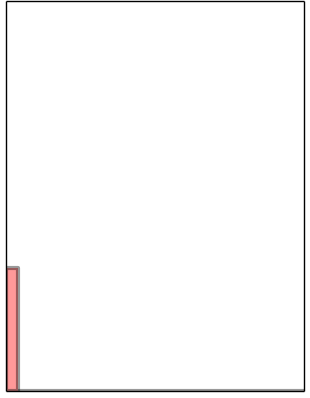
\includegraphics[scale=0.1]{p1.png}};
\node (plot) at (7.7,4.5) {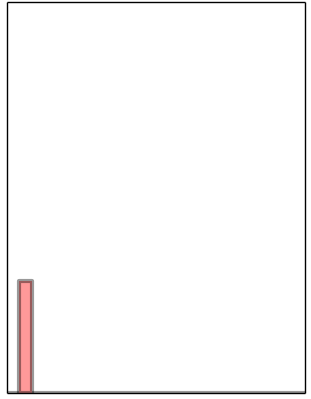
\includegraphics[scale=0.1]{p2.png}};
\node[text width=0.5cm] at (9.5,4) {\LARGE {.}};
\node[text width=0.5cm] at (10.5,4) {\LARGE {.}};
\node[text width=0.5cm] at (11.5,4) {\LARGE {.}};
\node (plot) at (12.7,4.5) {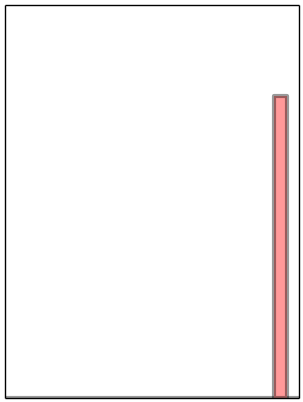
\includegraphics[scale=0.1]{p3.png}};
\node (plot) at (14.7,4.5) {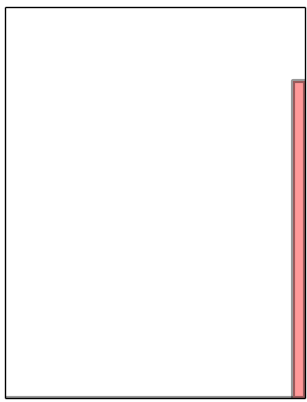
\includegraphics[scale=0.1]{p4.png}};
}

\onslide<6-> {
\node [neuron1] (neuron2) at (10,7) {$+$};
\draw[->]  (5.7,5.4) -- (neuron2);
\draw[->]  (7.7,5.4) -- (neuron2);

\node[text width=0.5cm] at (9.5,5.5) {\LARGE {.}};
\node[text width=0.5cm] at (10.5,5.5) {\LARGE {.}};
\node[text width=0.5cm] at (11.5,5.5) {\LARGE {.}};

\draw[->]  (12.7,5.4) -- (neuron2);
\draw[->]  (14.7,5.4) -- (neuron2);
\draw[->]  (neuron2) -- (10,8.8) ;
}
\node (plot) at (10,10.5) {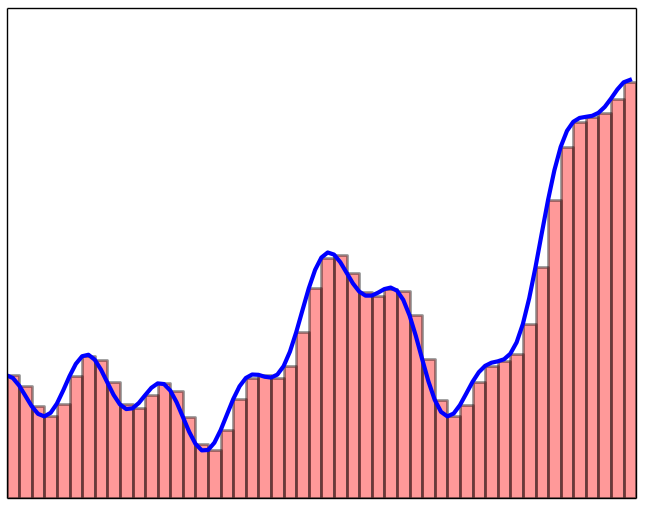
\includegraphics[width=7cm, height=2cm]{plot.png}};

\end{tikzpicture}
\end{overlayarea}



\column{0.5\textwidth}
\begin{overlayarea}{\textwidth}{\textheight}
\begin{itemize}
\item<1-> We make a few observations
\item<2-> All these ``tower'' functions are similar and only differ in their heights and positions on the x-axis
\item<3-> Suppose there is a black box which takes the original input ($x$) and constructs these tower functions
\item<5-> We can then have a simple network which can just add them up to approximate the function
\item<7-> Our job now is to figure out what is inside this blackbox
\end{itemize}
\end{overlayarea}
\end{columns}
\end{frame}


\begin{frame}
We will figure this out over the next few slides ...
\end{frame}

\begin{frame}
\begin{columns}
\column{0.5\textwidth}
\begin{overlayarea}{\textwidth}{\textheight}
\begin{onlyenv}
\only<0-44>{
\begin{figure}
    \includegraphics<1-2>[scale=0.25]{images/Plots/sig_2d/a_6}    
\foreach \n in {0,...,44} {%
    \pgfmathsetmacro\result{int(\n + 6)}
    \pgfmathsetmacro\t{int(\n + 3)}
    \includegraphics<\t>[scale=0.25]{images/Plots/sig_2d/a_\result}    
}
\end{figure}  
\foreach \n in {0,...,44} {%
    \pgfmathsetmacro\result{int(\n + 6)}
    \pgfmathsetmacro\t{int(\n + 3)}
    \only<\t>{$w = \result, b = 0, \t$}
}
}
\only<45->{
\begin{figure}
\foreach \n in {1,...,35} {%
    \pgfmathsetmacro\result{int(\n + 44)}
    \includegraphics<\result>[scale=0.25]{images/Plots/sig_2d/b_\n}    
}
\end{figure}  
\foreach \n in {1,...,35} {%
    \pgfmathsetmacro\result{int(\n + 44)}
    \only<\result>{$w = 50, b = \n $}
}
}
\end{onlyenv}
\end{overlayarea}



\column{0.5\textwidth}
\begin{overlayarea}{\textwidth}{\textheight}
\begin{itemize}
\item<1-> If we take the logistic function and set $w$ to a very high value we will recover the step function
\item<2-> Let us see what happens as we change the value of $w$ 
\item<45-> Further we can adjust the value of $b$ to control the position on the x-axis at which the function transitions from 0 to 1 
%\item Now lets see what we get by taking two such sigmoid functions (with different $b$s) and subtracting one from the other
%\item Voila! We have our tower function !!
%\item Let us see the neural network that gave us this tower function
\end{itemize}
\end{overlayarea}
\end{columns}
\end{frame}


\begin{frame}
\begin{columns}
\column{0.5\textwidth}
\begin{overlayarea}{\textwidth}{\textheight}

\tikzstyle{neuron}=[circle,draw=red!50,fill=red!10, thick,minimum size=10mm]
\tikzstyle{neuron1}=[circle,draw=blue!50,fill=cyan!10, thick,minimum size=10mm]
\begin{tikzpicture}

\node (plot) at (0,10) {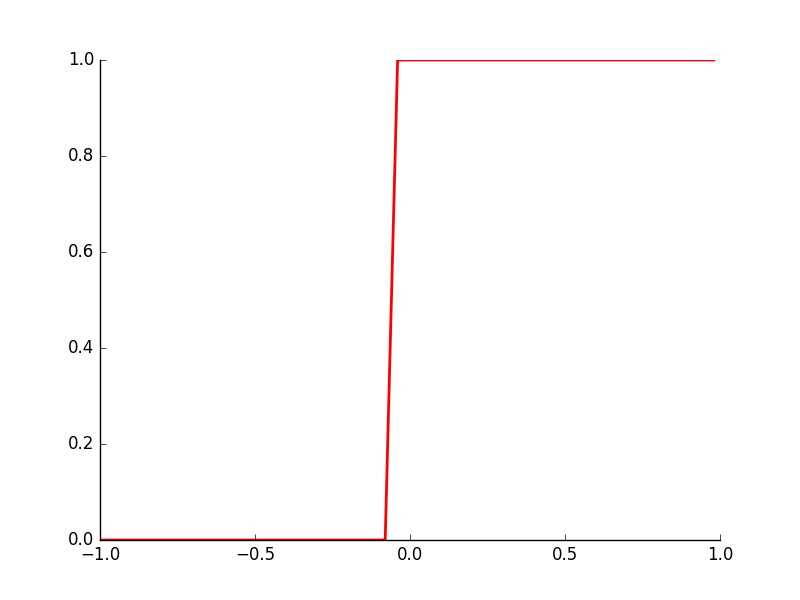
\includegraphics[width=4cm,height=4cm]{./images/Plots/1}};

\node (plot) at (4,10) {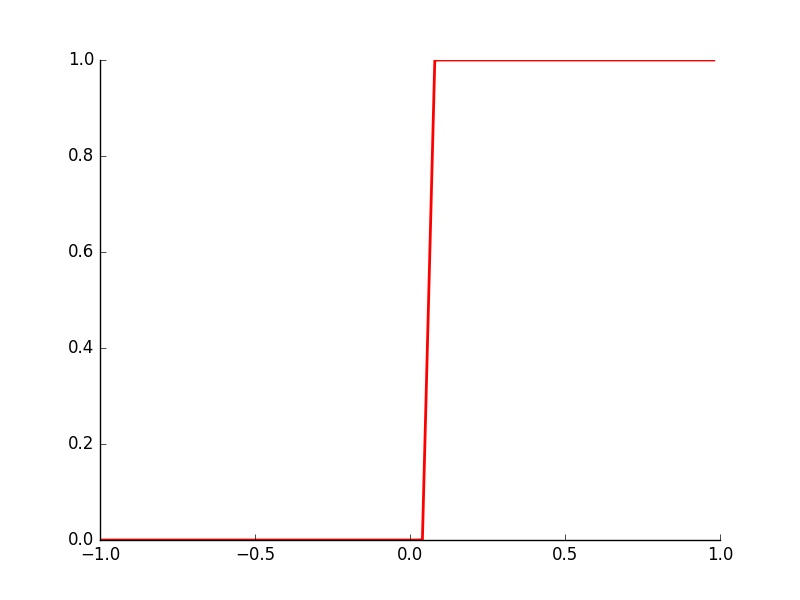
\includegraphics[width=4cm,height=4cm]{./images/Plots/2}};

\onslide<3->{\node (plot) at (2,6) {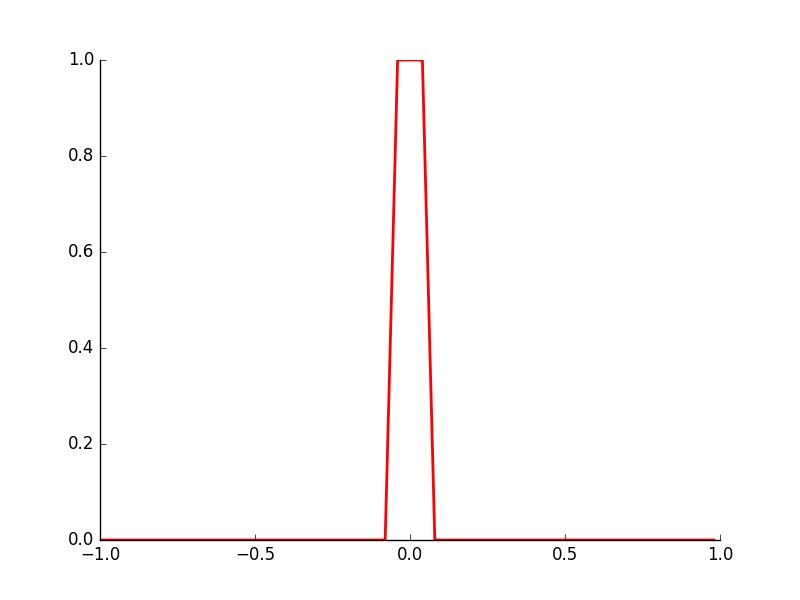
\includegraphics[width=4cm,height=4cm]{./images/Plots/tower}};}
\onslide<2->{\draw[line width=0.2mm](2, 10) -- (2.2,10);}
%\draw[line width=0.2mm](2.1,10.1)--(2.1,9.9);
\onslide<3->{\draw[line width=0.2mm](2,8) -- (2.2,8);}
\onslide<3->{\draw[line width=0.2mm](2,8.1)--(2.2,8.1);}
\end{tikzpicture}
\end{overlayarea}


\column{0.5\textwidth}
\begin{overlayarea}{\textwidth}{\textheight}
\begin{itemize}
\item Now lets see what we get by taking two such sigmoid functions (with different $b$s) and subtracting one from the other
\item<4-> Voila! We have our tower function !!
\end{itemize}
\end{overlayarea}
\end{columns}
\end{frame}

\begin{frame}
\begin{itemize}
\item Can we come up with a neural network to represent this operation of subtracting one sigmoid function from another ?
\end{itemize}
\end{frame}


\begin{frame}
\begin{figure}
    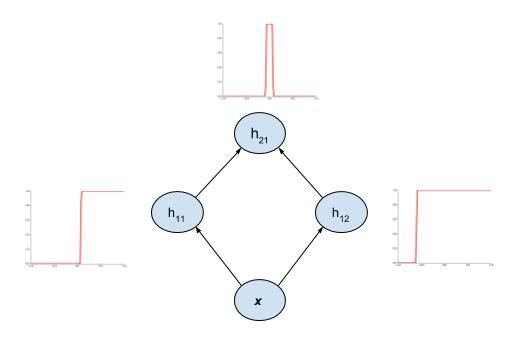
\includegraphics[scale=0.5]{images/Plots/nn2d}    
\end{figure}
\end{frame}

%\begin{frame}
%Later on in the assignment you will show that you could have done with just one hidden layer instead of two! 
%\end{frame}

\begin{frame}
What if we have more than 1 input ?
\end{frame}


\begin{frame}
\begin{columns}
\column{0.5\textwidth}
\begin{overlayarea}{\textwidth}{\textheight}
\begin{onlyenv}
\only<0-26>{
\begin{figure}
    \includegraphics<1-3>[scale=0.25]{images/Plots/one/2}    
\foreach \n in {4,...,25} {%
    \pgfmathsetmacro\result{int(\n - 1)}
    \includegraphics<\n>[scale=0.25]{images/Plots/one/\result}    
}
    \includegraphics<26>[scale=0.25]{images/Plots/one/25}    
\end{figure} 
\foreach \n in {3,...,25} {%
    \pgfmathsetmacro\result{int(\n - 1)}
    \only<\n>{$w_1 = \result, w_2 = 0, b = 0 $}
}
}
\only<27->{
\begin{figure}
\foreach \n in {0,...,9} {%
    \pgfmathsetmacro\result{int(\n + 27)}
    \includegraphics<\result>[scale=0.25]{images/Plots/two/\n}    
}
\end{figure}  
\foreach \n in {0,...,9} {%
    \pgfmathsetmacro\result{int(\n + 27)}
    \pgfmathsetmacro\b{int(\n * 5)}
    \only<\result>{$w_1 = 25, w_2 = 0, b = \b $}
}
}
\end{onlyenv}
\end{overlayarea}



\column{0.5\textwidth}
\begin{overlayarea}{\textwidth}{\textheight}
\begin{itemize}
\item<1-> This is what a 3-dimensional sigmoid looks like 
\item<2-> We need to figure out how to get a 3-dimensional tower
\item<3-> First, let us set $w_2$ to 0 and see if we can get a two dimensional step function
\item<26-> What would happen if we change $b$ ? 
%\item Now lets see what we get by taking two such sigmoid functions (with different $b$s) and subtracting one from the other
%\item Voila! We have our tower function !!
%\item Let us see the neural network that gave us this tower function
\end{itemize}
\end{overlayarea}
\end{columns}
\end{frame}

\begin{frame}
\begin{columns}
\column{0.5\textwidth}
\begin{overlayarea}{\textwidth}{\textheight}

\tikzstyle{neuron}=[circle,draw=red!50,fill=red!10, thick,minimum size=10mm]
\tikzstyle{neuron1}=[circle,draw=blue!50,fill=cyan!10, thick,minimum size=10mm]
\begin{tikzpicture}

\node (plot) at (0,10) {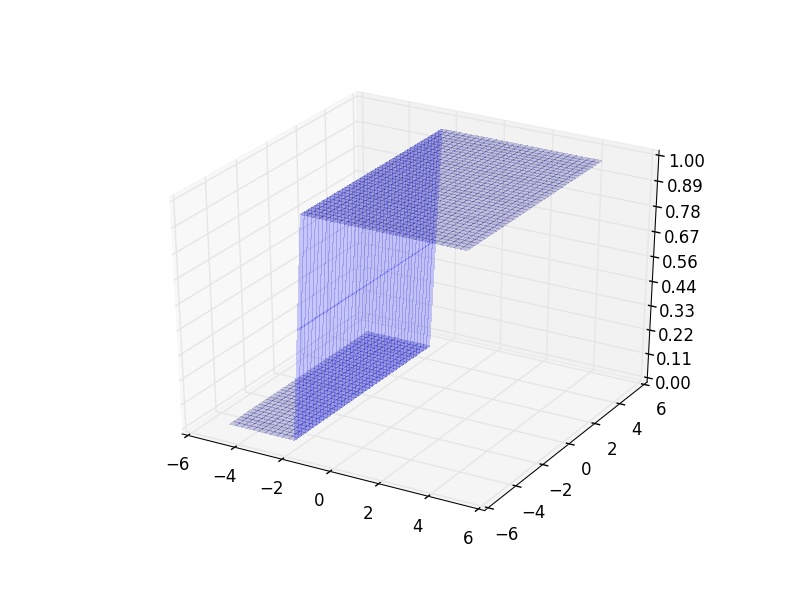
\includegraphics[width=4cm,height=4cm]{./images/Plots/three/x1}};

\node (plot) at (4,10) {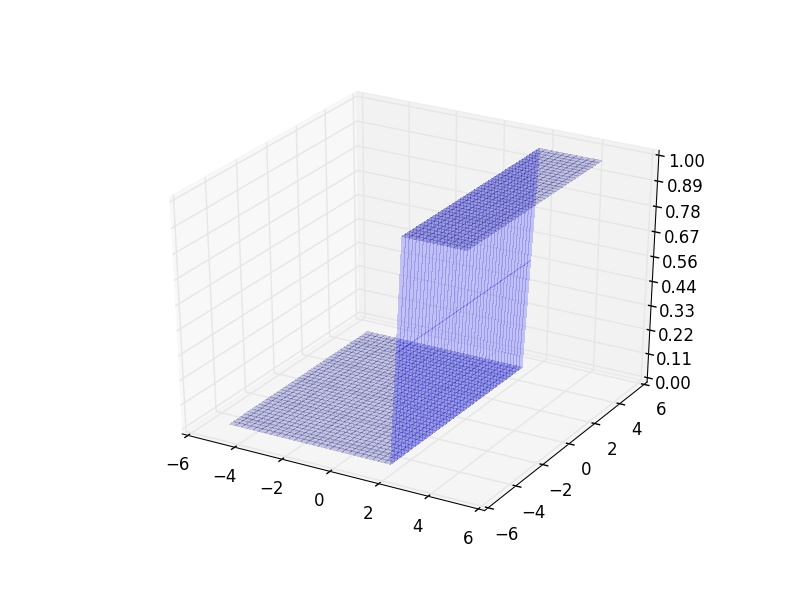
\includegraphics[width=4cm,height=4cm]{./images/Plots/three/x2}};

\onslide<3->{\node (plot) at (2,6) {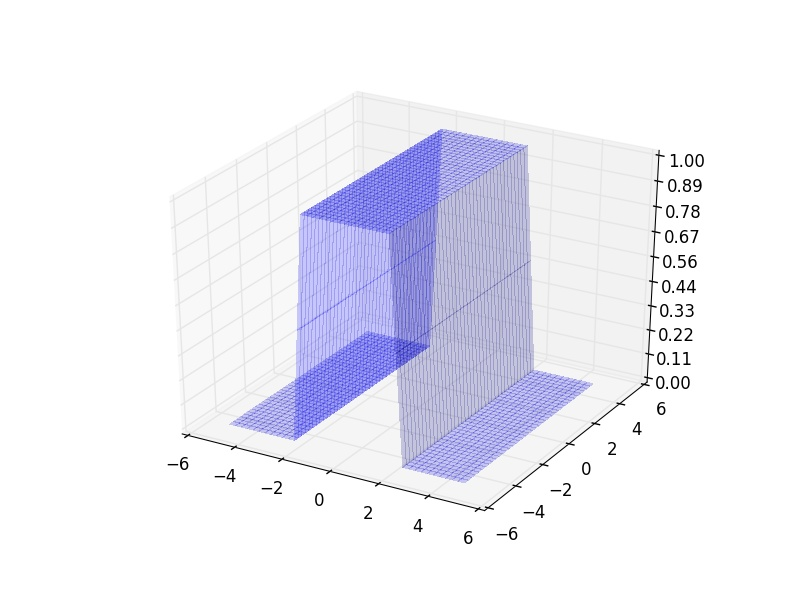
\includegraphics[width=4cm,height=4cm]{./images/Plots/three/xjoin}};}
\onslide<2->{\draw[line width=0.2mm](2, 10) -- (2.2,10);}
%\draw[line width=0.2mm](2.1,10.1)--(2.1,9.9);
\onslide<3->{\draw[line width=0.2mm](2,8) -- (2.2,8);}
\onslide<3->{\draw[line width=0.2mm](2,8.1)--(2.2,8.1);}
\end{tikzpicture}
\end{overlayarea}


\column{0.5\textwidth}
\begin{overlayarea}{\textwidth}{\textheight}
\begin{itemize}
\item<1-> What if we take two such step functions (with different $b$ values) and subtract one from the other
\item<4-> We still don't get a tower (or we get a tower which is open from two sides)
%\item Now lets see what we get by taking two such sigmoid functions (with different $b$s) and subtracting one from the other
%\item Voila! We have our tower function !!
%\item Let us see the neural network that gave us this tower function
\end{itemize}
\end{overlayarea}
\end{columns}
\end{frame}


\begin{frame}
\begin{columns}
\column{0.5\textwidth}
\begin{overlayarea}{\textwidth}{\textheight}
\begin{onlyenv}
\only<0-26>{
\begin{figure}
    \includegraphics<1-3>[scale=0.25]{images/Plots/five/2}    
\foreach \n in {4,...,25} {%
    \pgfmathsetmacro\result{int(\n - 1)}
    \includegraphics<\n>[scale=0.25]{images/Plots/five/\result}    
}
    \includegraphics<26>[scale=0.25]{images/Plots/five/25}    
\end{figure} 
\foreach \n in {3,...,25} {%
    \pgfmathsetmacro\result{int(\n - 1)}
    \only<\n>{$w_1 = 0, w_2 = \result, b = 0 $}
}
}
\only<27->{
\begin{figure}
\foreach \n in {0,...,9} {%
    \pgfmathsetmacro\result{int(\n + 27)}
    \includegraphics<\result>[scale=0.25]{images/Plots/six/\n}    
}
\end{figure}  
\foreach \n in {0,...,9} {%
    \pgfmathsetmacro\result{int(\n + 27)}
    \pgfmathsetmacro\b{int(\n * 5)}
    \only<\result>{$w_1 = 0, w_2 = 25, b = \b $}
}
}
\end{onlyenv}
\end{overlayarea}



\column{0.5\textwidth}
\begin{overlayarea}{\textwidth}{\textheight}
\begin{itemize}
\item<1-> Now let us set $w_1$ to 0 and adjust $w_2$ to get a 3-dimensional step function with a different orientation
\item<26-> And now we change $b$ 
\end{itemize}
\end{overlayarea}
\end{columns}
\end{frame}


\begin{frame}
\begin{columns}
\column{0.5\textwidth}
\begin{overlayarea}{\textwidth}{\textheight}

\tikzstyle{neuron}=[circle,draw=red!50,fill=red!10, thick,minimum size=10mm]
\tikzstyle{neuron1}=[circle,draw=blue!50,fill=cyan!10, thick,minimum size=10mm]
\begin{tikzpicture}

\node (plot) at (0,10) {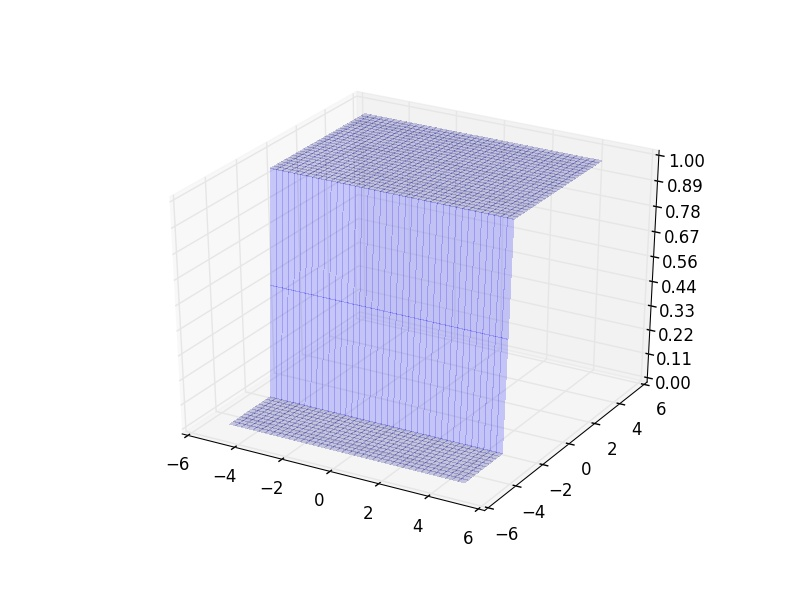
\includegraphics[width=4cm,height=4cm]{./images/Plots/three/y1}};

\node (plot) at (4,10) {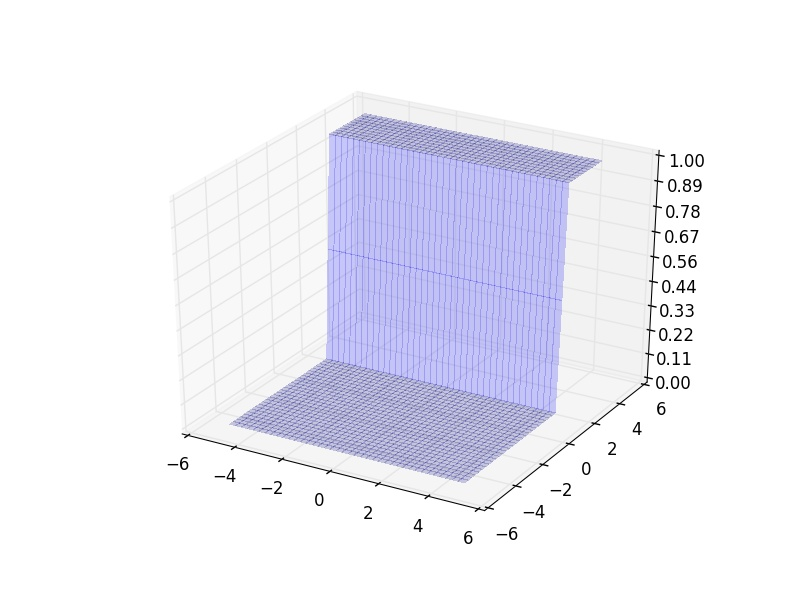
\includegraphics[width=4cm,height=4cm]{./images/Plots/three/y2}};

\onslide<3->{\node (plot) at (2,6) {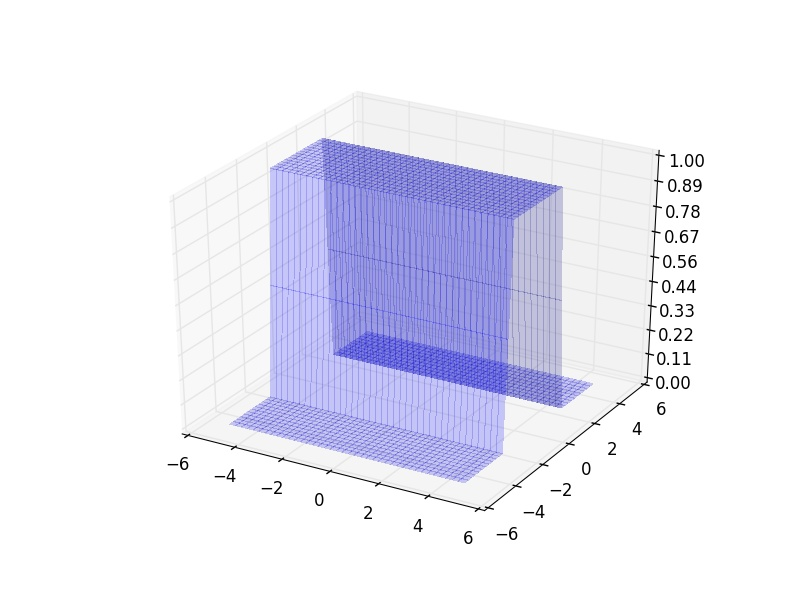
\includegraphics[width=4cm,height=4cm]{./images/Plots/three/yjoin}};}
\onslide<2->{\draw[line width=0.2mm](2, 10) -- (2.2,10);}
%\draw[line width=0.2mm](2.1,10.1)--(2.1,9.9);
\onslide<3->{\draw[line width=0.2mm](2,8) -- (2.2,8);}
\onslide<3->{\draw[line width=0.2mm](2,8.1)--(2.2,8.1);}
\end{tikzpicture}
\end{overlayarea}


\column{0.5\textwidth}
\begin{overlayarea}{\textwidth}{\textheight}
\begin{itemize}
\item<1-> Again, what if we take two such step functions (with different $b$ values) and subtract one from the other
\item<4-> We still don't get a tower (or we get a tower which is open from two sides)
\item<5-> Notice that this open tower has a different orientation from the previous one
%\item Now lets see what we get by taking two such sigmoid functions (with different $b$s) and subtracting one from the other
%\item Voila! We have our tower function !!
%\item Let us see the neural network that gave us this tower function
\end{itemize}
\end{overlayarea}
\end{columns}
\end{frame}


\begin{frame}
\begin{columns}
\column{0.5\textwidth}
\begin{overlayarea}{\textwidth}{\textheight}

\only<1-5>{
\tikzstyle{neuron}=[circle,draw=red!50,fill=red!10, thick,minimum size=10mm]
\tikzstyle{neuron1}=[circle,draw=blue!50,fill=cyan!10, thick,minimum size=10mm]
\begin{tikzpicture}

\node (plot) at (0,10) {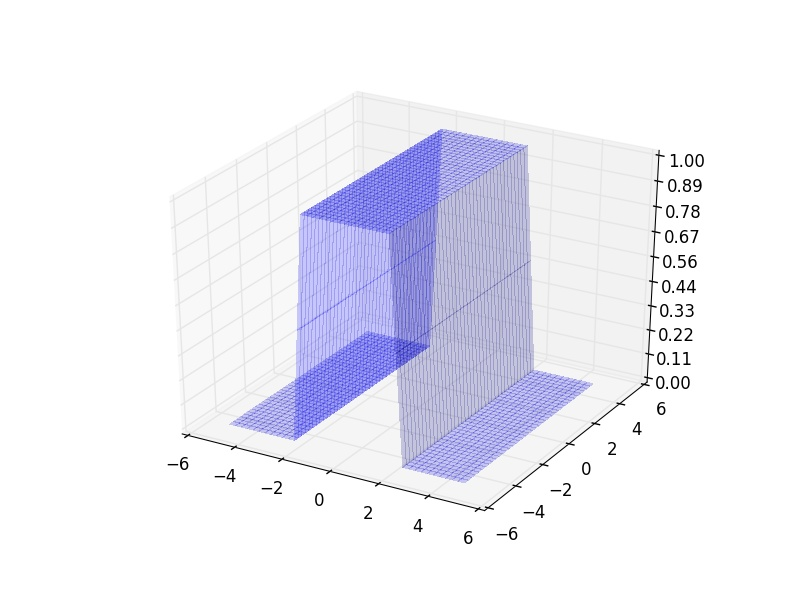
\includegraphics[width=4cm,height=4cm]{./images/Plots/three/xjoin}};

\node (plot) at (4,10) {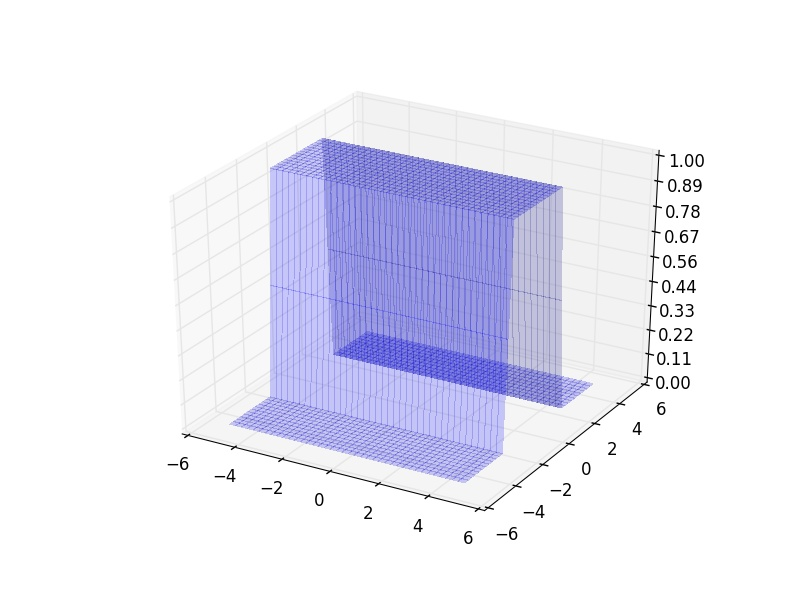
\includegraphics[width=4cm,height=4cm]{./images/Plots/three/yjoin}};

\onslide<3->{\node (plot) at (2,6) {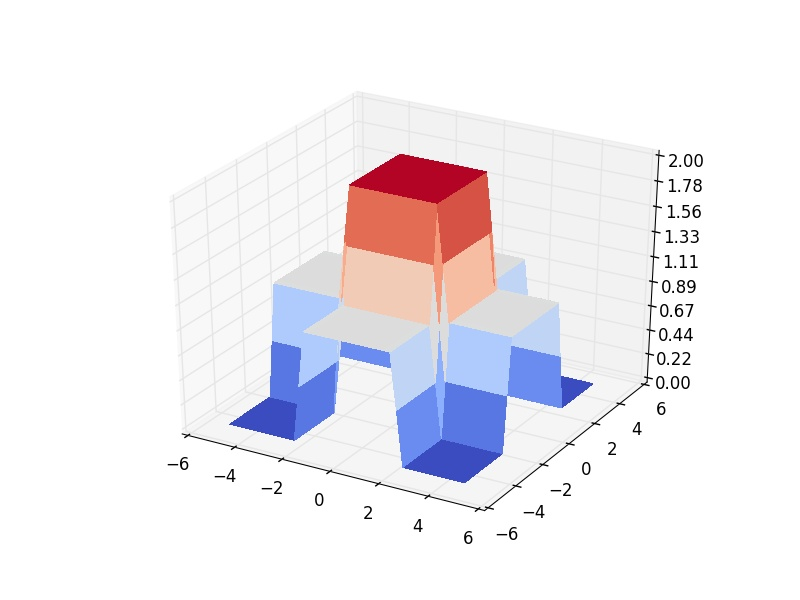
\includegraphics[width=4cm,height=4cm]{./images/Plots/three/xpyjoin}};}
\onslide<2->{\draw[line width=0.2mm](2, 10) -- (2.2,10);}
%\draw[line width=0.2mm](2.1,10.1)--(2.1,9.9);
\onslide<3->{\draw[line width=0.2mm](2,8) -- (2.2,8);}
\onslide<3->{\draw[line width=0.2mm](2,8.1)--(2.2,8.1);}
\end{tikzpicture}
}
\only<6->{
\begin{figure}
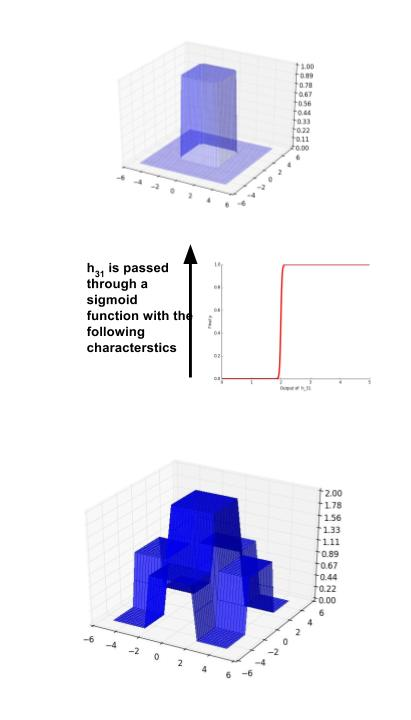
\includegraphics[scale=0.3]{./images/Plots/four/t_add}
\end{figure}

}
\end{overlayarea}


\column{0.5\textwidth}
\begin{overlayarea}{\textwidth}{\textheight}
\begin{itemize}
\item<1-> Now what will we get by adding two such open towers ?
\item<4-> We get a tower standing on an elevated base
\item<5-> We can now pass this output through another sigmoid neuron to get the desired tower !
\item<7-> We can now approximate any function by summing up many such towers
%\item Now lets see what we get by taking two such sigmoid functions (with different $b$s) and subtracting one from the other
%\item Voila! We have our tower function !!
%\item Let us see the neural network that gave us this tower function
\end{itemize}
\end{overlayarea}
\end{columns}
\end{frame}

\begin{frame}
\begin{columns}
\column{0.5\textwidth}
\begin{overlayarea}{\textwidth}{\textheight}
\begin{figure}
    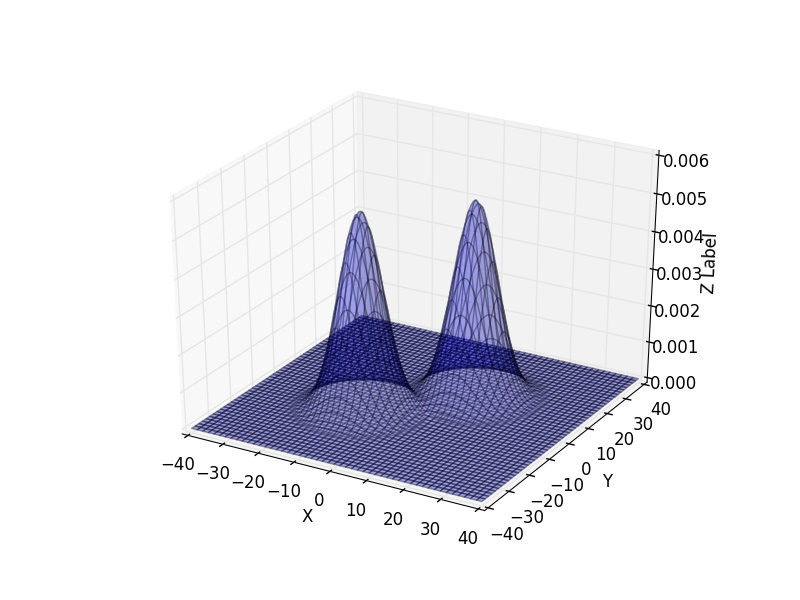
\includegraphics[scale=0.25]{images/Plots/2bells}    
\end{figure}

\end{overlayarea}

\column{0.5\textwidth}
\begin{overlayarea}{\textwidth}{\textheight}
\begin{itemize}
\item For example, we could approximate the following function using a sum of several towers 
\end{itemize}
\end{overlayarea}
\end{columns}
\end{frame}

\begin{frame}
\begin{itemize}
\item Can we come up with a neural network to represent this entire procedure of constructing a 3 dimensional tower ?
\end{itemize}
\end{frame}

\begin{frame}
\begin{figure}
    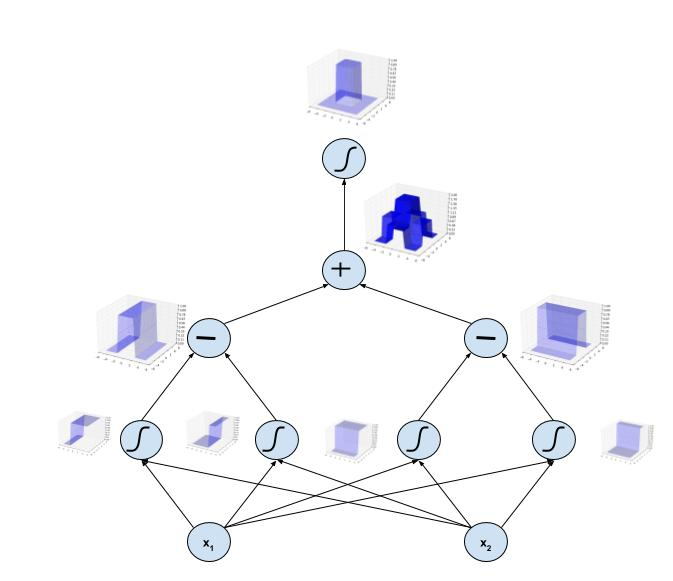
\includegraphics[scale=0.25]{images/Plots/nn_step}    
\end{figure}
\end{frame}

\begin{frame}
\begin{figure}
    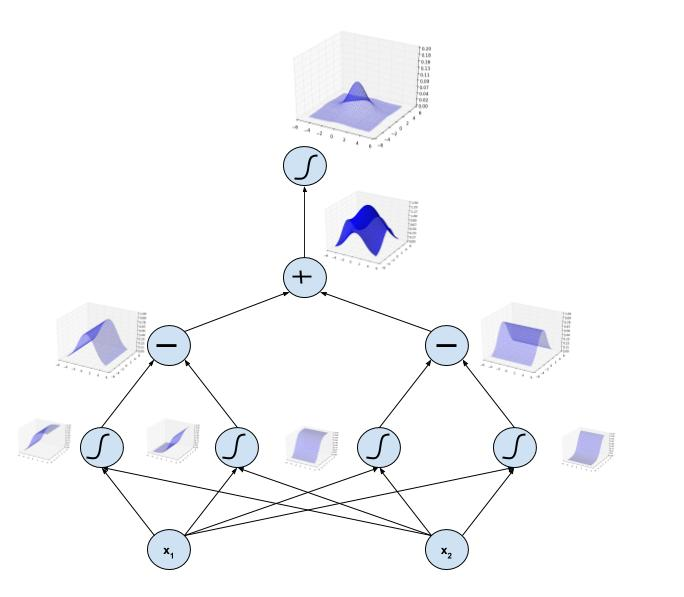
\includegraphics[scale=0.25]{images/Plots/nn_g}    
\end{figure}
\end{frame}


\begin{frame}
\begin{block}{Think}
\begin{itemize}
\item For 1 dimensional input we needed 2 neurons to construct a tower
\item For 2 dimensional input we needed 4 neurons to construct a tower
\item How many neurons will you need to construct a tower in $n$ dimensions ?
\end{itemize}
\end{block}
\end{frame}

\begin{frame}
\begin{block}{Time to retrospect}
\begin{itemize}
\item Why do we care about approximating any arbitrary function ?
\item Can we tie all this back to the classification problem that we have been dealing with ?
\end{itemize}
\end{block}
\end{frame}


\begin{frame}
\begin{columns}
\column{0.5\textwidth}
\begin{overlayarea}{\textwidth}{\textheight}

\begin{figure}
    \includegraphics<1-2>[scale=0.10]{images/Plots/scatter}    
    \includegraphics<3->[scale=0.10]{images/Plots/sig1.png}    
\end{figure}
\vspace{-0.2in}
\begin{itemize}
\item We are interested in separating the blue points from the red points
\item<2-> Suppose we use a single sigmoidal neuron to approximate the relation between $x = [x_1, x_2]$ and $y$
\item<4-> Obviously, there will be errors (some blue points get classified as 1 and some red points get classified as 0) 
%This will what a single neuron will give us $y = \frac{1}{1 + e^{-(w_2*x_2 + w_1*x_1 + w_0)}}$
\end{itemize}

\end{overlayarea}



\column{0.5\textwidth}
\begin{overlayarea}{\textwidth}{\textheight}
\begin{figure}
    \includegraphics<5->[scale=0.10]{images/Plots/g2.png}    
\end{figure}
\vspace{-0.2in}

\begin{itemize}
\item<5-> This is what we actually want
\item<6-> The illustrative proof that we just saw tells us that we can have a neural network with two hidden layers which can approximate the above function by a sum of towers
\item<7-> Which means we can have a neural network which can exactly separate the blue points from the red points !!
\end{itemize}
\end{overlayarea}
\end{columns}
\end{frame}


\if 0
\begin{frame}
\begin{columns}
\column{0.5\textwidth}
\begin{overlayarea}{\textwidth}{\textheight}
\end{overlayarea}



\column{0.5\textwidth}
\begin{overlayarea}{\textwidth}{\textheight}
\begin{itemize}
\item 1 
\end{itemize}
\end{overlayarea}
\end{columns}
\end{frame}
perceptron function and sigmoid function (continuous differentiable)
terminology b instead of w0
something about different loss functions
something about non-linearities
bigger scheme of things
representation power
the hat diagrams
add assignment for two layered network

Column1: This is what a single neural network can do
Column2: This is what we want

What is the data is even more difficult (show several bumps)

The function y can be seen as an addition of several such small bump functions (show it visually)



Proposition: if we can have a network which can approximate sa bump then we can combine several such networks together to

Question: Can we have a network of neurons which can represent such arbitrary functions
Side by side definitions of boolean and real UAT
Caveats: it does not tell us anything about the number of neurons in the layer


#Study MAterial
Sigmoid function
Code for plotting sigmoid function
Can be interpreted as a probablity
\fi

\end{document}


